\documentclass{article}

\usepackage[left=1.5in, right=1.5in, top=1in, bottom=1in]{geometry}

\usepackage{setspace}
\doublespacing

\usepackage{ragged2e}
\justifying

\usepackage{tikz}
\usepackage{lscape}
\usepackage{graphicx}
\usepackage{amsmath}
\usepackage{amssymb}
\usepackage{hyperref}
\usepackage{array}

\usepackage{graphicx}
\graphicspath{ {./img/} }

\usepackage[backend=biber]{biblatex}
\bibliography{sources.bib}

\title{Comparing Models of Delta-Notch Signalling}  
\author{Riley Wheadon, Edwin Huras, Ziyi Zhuang}

\begin{document}

\maketitle

\section*{Abstract}

The Delta-Notch signalling pathway plays a crucial role in driving the differentiation of initially homogeneous cells in a variety of biological systems.
In this paper, we present a simple biological model of Delta-Notch signalling and investigate it using three mathematical formalisms: ODE, SDE, and agent-based.
Using the Kolmogorov forward equations, we show that the agent-based model converges to the ODE model in expectation.
We also demonstrate that the SDE and agent-based models can produce cell differentiation even from identical initial conditions.
Finally, we study the effect of parameters such as stochastic noise, domain shape, and boundary conditions on the behaviour of our models.
Our findings provide insight into how modelling formalisms can affect simulations of the Delta-Notch signalling network with significant implications for future research. 

\section*{Introduction}

Cell differentiation is essential for the formation of structure in complex organisms.
However, only a few signalling pathways are responsible for this important function \cite{bray_notch_2006}.
One of these pathways is the Delta-Notch signalling network, which has been shown to drive neurogenesis in vertebrates by determining which cells adopt neural and glial fates. 
Furthermore, mutations in Notch activity has been shown to be a contributing factor to many cancers \cite{bray_notch_2006}.
The Delta-Notch signalling network is unique because its ligands Delta and Jagged are transmembrane proteins.
This means that Delta-Notch signalling is largely restricted to neighbouring cells. 
However, new findings suggest that cellular protrusions can allow a small fraction of Delta-Notch signals to travel longer distances \cite{berkemeier_coupling_2023}.

\begin{figure}[ht]
  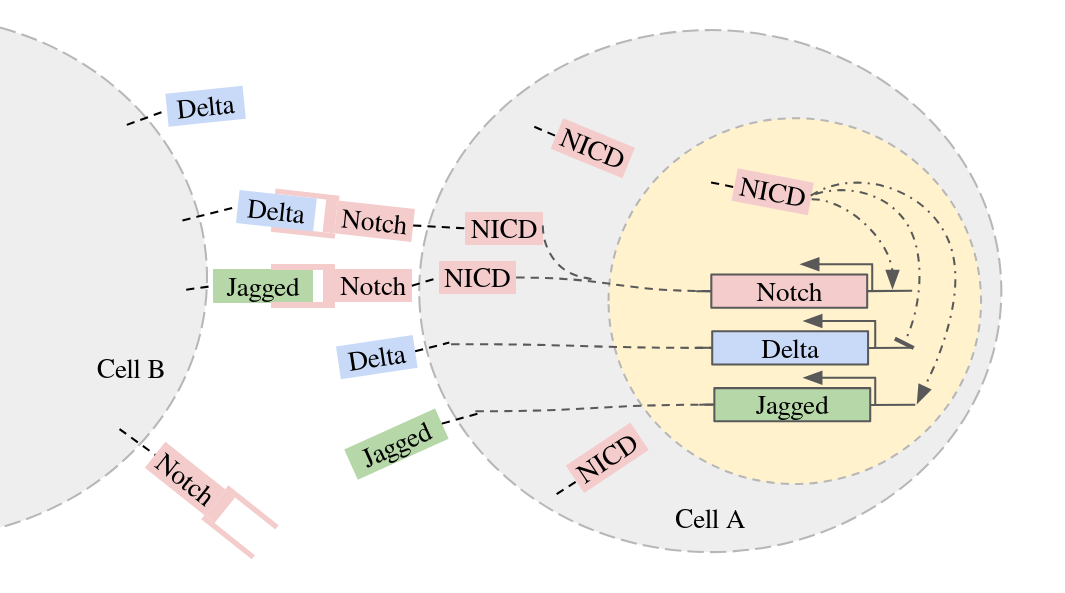
\includegraphics[width=\textwidth]{img/signalling-network.png}
  \caption{
Illustration of the Delta-Notch signalling network.
Binding of the Delta and Jagged ligands from cell $B$ to the Notch receptors on cell $A$ results in the \emph{cleavage} (removal) of both the ligand and receptor \cite{bray_notch_2006}.
This interaction triggers the release of NICD (Notch Intracellular Domain) in cell $A$, which \emph{promotes} Notch, \emph{inhibits} Delta, and \emph{promotes} Jagged.
It is also possible for a Delta ligand to bind to a Notch receptor on the same cell. This phenomenon, known as \emph{cis-inhibition}, cleaves the Notch receptor but does not release NICD.
  }
\end{figure}

Interactions between Delta, Notch, and Jagged on the cell membrane cause some cells to adopt a low-Notch state (the \emph{primary fate}) and others to adopt a high-Notch state (the \emph{secondary fate}).
Typically, primary and secondary fated cells form an alternating pattern.
Then, through other signalling networks, the primary and secondary fated cells adopt different characteristics depending on the organism and organ. 

The model of Delta-Notch signalling proposed by Collier et al. \cite{collier_pattern_1996} is one of the seminal works in the field.
Through their ODE model, Collier et al. show that if a linear array of cells is given zero-flux boundary conditions, a pattern of alternating cell fates arises on the outside edges before gradually spreading inwards towards the center of the domain.
Additionally, Collier et al. show that their model exhibits different ratios of primary to secondary fated cells depending on the parameters when simulated on a two-dimensional hexagonal lattice. 
While these qualitative results are important, Collier et al. use many simplifications that make it difficult to identify how individual chemical reactions are captured by the model.
For instance, production of activated Notch (NICD) is exclusively a function of the Delta concentration in neighbouring cells, without regard for the concentration of Notch receptors.
This violates the mass-balance equations, since we now know that the quantity of Notch receptors changes dynamically in response to the concentration of Delta ligands in nearby cells.
The ODE model of Delta-Notch signalling proposed by Boareto et al. \cite{boareto_jaggeddelta_2015} is built on a more modern understanding of the biochemistry of the system.
Their model respects the mass-balance equations and explicitly includes binding rate and decay rates. 
The Boareto et al. model also assumes that production of Notch is an increasing hill function of NICD while production of Delta is a decreasing hill function of NICD, a useful simplification that we will also use.
However, Boareto et al. \cite{boareto_jaggeddelta_2015} only analyze their model on a two-cell domain, which makes it difficult to generalize their results to larger groups of cells.

In this paper, we develop three models of the Delta-Notch signalling network. 
Our first model is an agent-based simulation of individual Delta, Notch, and NICD molecules. 
While this model precisely simulates the reaction kinetics, it is impossible to analyze analytically and slow to simulate computationally.
Then, we define two models based on differential equations.
The ODE model is a deterministic representation of the approximate reaction kinetics, while the SDE model includes noise terms to better replicate the agent-based model.
To connect our agent-based and ODE models, we use the Kolmogorov forward equations, taking their expectation and applying the law of total expectation to derive a system of ODEs for the expected molecular counts (see Appendix \ref{sec:kfe}, \ref{sec:theoretical-justification}).
This calculation relies on the assumption that the propensity functions are approximately linear or that fluctuations around the mean are small, which holds when molecule numbers are large.
Under this assumption, evaluating the propensity functions at the expected state recovers our deterministic ODE model after appropriate scaling.
We then compare all three models with each other using a combination of analytical and computational methods in a variety of different domains.
Furthermore, we show that our models qualitatively replicate the results of Collier et al. \cite{collier_pattern_1996}. 

\section*{Methods}

From the literature \cite{collier_pattern_1996, boareto_jaggeddelta_2015}, we assume Notch ($N$) receptor production has the form $H^{+}(I) = n_{m}I^2/(n_{0}^2 + I^2)$ where $I$ is the NICD concentration and $n_{m}, n_{0}$ are hill function parameters.
Similarly, we assume production of the Delta ligand ($D$) is governed by a decreasing hill function of the form $H^{-}(I) = d_{m}d_{0}^2/(d_{0}^2 + I^2)$.
Furthermore, we will assume that Notch and Delta both have decay rate $\gamma$.
The variable $k_{T}$ will denote the binding rate between Notch receptors and Delta ligands.
$\gamma_{I}$ is the decay rate of NICD.
We will also assume that there is no cis-inhibition and no Jagged ligand. 

\begin{table}[!htp]
\centering
\begin{tabular}{|m{8em}|m{5em}|m{20em}|} 
 \hline
 Reaction & Rate & Description \\ 
 \hline
 $N_{A} + D_{B} \rightarrow I_{A}$ & 
 $k_{T} N_{A}D_{B}$ &
 A Notch receptor from cell $A$ binds to a Delta ligand from cell $B$, triggering the release of NICD in cell $A$. \\
 \hline
 $N_{A} \rightarrow \emptyset$ & 
 $\gamma N_{A}$ & 
 A Notch receptor from cell $A$ decays. \\
 \hline
 $D_{A} \rightarrow \emptyset$ & 
 $\gamma D_{A}$ & 
 A Delta receptor from cell $A$ decays. \\
 \hline
 $I_{A} \rightarrow \emptyset$ &
 $\gamma_{I} I_{A}$ &
 A NICD molecule from cell $A$ decays.  \\
 \hline
 $\emptyset \rightarrow N_{A}$ & 
 $H^{+}(I_{A})$ &
 A Notch receptor in cell $A$ is produced \\
 \hline
 $\emptyset \rightarrow D_{A}$ &
 $H^{-}(I_{A})$ &
 A Delta ligand in cell $A$ is produced \\
 \hline
\end{tabular}
\caption{
  A list of possible reactions and their rates in a cell $A$ with neighbour $B$.
  Since there are $6$ possible reactions per cell, a system with $n$ cells will have $6n$ possible reactions.
  In the Reaction column, $N_A$, $D_B$, and $I_A$ represent one Notch, Delta, and NICD, respectively. In the Rate column, $N_A$, $D_B$, and $I_A$ refer to the number of Notch molecules in cell A, Delta in cell B, and NICD in cell A, respectively.
}
\label{tb:reactions}
\end{table}

We will assume that reaction times follow a Poisson point process.
Suppose $E$ is the set of all possible reaction events (the $6$ reactions above for all cells).
Furthermore, let $|E| = N$ be the number of possible reactions.
For each event, let $X_{i} \sim \text{Exp}(\lambda_{i})$ denote the time until the next event of type $i$, where $1 \leq i \leq N$.
Then, the waiting time $T$ in between any two events is given by the formula in Equation \ref{eq:waiting-time} due to the memoryless property.

\begin{equation}
T = \text{min} \{ X_{1}, \dots, X_{N} \} \sim \text{Exp}\left( \sum_{i = 1}^{N} \lambda_{i} \right) 
\label{eq:waiting-time}
\end{equation}

To simulate the individual reactions, we can use Gillespie's algorithm.
This is the agent-based model.
Details of the computational implementation can be found in Appendix \ref{sec:gillespie}.
In expectation, the agent-based model converges to the system of ordinary differential equations shown in Equation \ref{eq:deterministic}.
A proof of this fact can be found in Appendix \ref{sec:theoretical-justification}.
This is the ODE model, which is described below for a single cell in a two-cell system.
However, this model can be extended to arbitrary domains by defining equations $dN_{i}/dt$, $dD_{i}/dt$, and $dI_{i}/dt$ for each $i \in \{ 1, \dots, n \}$, where $n$ is the number of cells.
In a domain of arbitrary size, $N_{ext}$ and $D_{ext}$ are the average Notch and Delta concentrations over all neighbours.

\begin{equation}
\begin{aligned}
  \frac{dN}{dt} &= \frac{n_{m}I^2}{n_{0}^2 + I^2} - k_{T}ND_{ext} - \gamma N \\[5pt]
  \frac{dD}{dt} &= \frac{d_{m}d_{0}^2}{d_{0}^2 + I^2} - k_{T}DN_{ext} - \gamma D \\[5pt]
  \frac{dI}{dt} &= k_{T}ND_{ext} - \gamma_{I}I
\end{aligned}
\label{eq:deterministic}
\end{equation}

This model is a simplification of the model by Boareto et al. \cite{boareto_jaggeddelta_2015}.
However, to more directly compare our results with those of Collier et al. \cite{collier_pattern_1996}, we chose to ignore Jagged and cis-inhibition.
Adding NICD, which was absent from Collier et al., was necessary for the assignment of probabilities to each reaction event.
An analysis of the system of ODEs in Equation \ref{eq:deterministic} for fixed values of $N_{ext}, D_{ext}$ reveals an $N = 0$ steady state (the \emph{primary fate}) for all parameter values.
There is also a high Notch steady state (the \emph{secondary fate}) which emerges from a fold bifurcation when $D_{ext}$ is sufficiently large.
See Appendix \ref{sec:bifurcation} for more information.

To capture the inherent randomness in receptor-ligand interactions while maintaining computational efficiency, we implement a stochastic differential equation (SDE) model based on the Langevin equation formalism.
This approach represents an intermediate level of detail between the ODE model and the fully discrete agent-based model.
Starting from the ODE model described in Equation \ref{eq:deterministic}, we incorporate stochastic fluctuations by adding noise terms proportional to the square root of the reaction rates to get Equation \ref{eq:stochastic}.

\begin{equation}
\begin{aligned}
  dN &= \left( \frac{n_{m}I^2}{n_{0}^2 + I^2} - k_{T}ND_{ext} - \gamma N \right) dt + \sigma \cdot N \cdot dW_{N} \\[5pt]
  dD &= \left( \frac{d_{m}d_{0}^2}{d_{0}^2 + I^2} - k_{T}DN_{ext} - \gamma D \right)  dt + \sigma \cdot D \cdot dW_{D}  \\[5pt]
  dI &= \left( k_{T}ND_{ext} - \gamma_{I}I \right) dt + \sigma \cdot I \cdot dW_{I}
\end{aligned}
\label{eq:stochastic}
\end{equation}

In Equation \ref{eq:stochastic}, $dW_N$, $dW_D$, and $dW_I$ are independent Wiener processes representing white noise.
The structure of the noise terms follows from the assumption that noise in each reaction channel is proportional to the current concentration of those molecules.
To implement the ODE and SDE models computationally, we employed the Euler-Maruyama method with time step $dt$.
The deterministic increment calculated first, and then the Wiener increments are sampled from a normal distribution with mean $0$ and standard deviation $\sqrt{dt}$.
Then, each Wiener increment is scaled by its respective variable and added to the deterministic increment.

\section*{Results}

\subsection*{Two-Cell Domains}

Collier et al. \cite{collier_pattern_1996} observed cell differentiation in their ODE model under small initial perturbations on a two-cell domain.
In our first experiment, we attempted to replicate this result under all three modelling formalisms.
Since the SDE and agent-based models are stochastic, we did not apply an initial perturbation to them.
For the ODE model, which is deterministic, we perturbed the initial Notch concentration by a factor of $X$, where $X$ is sampled from a $\mathcal{N}(1, 0.1)$ random variable.
The results of this experiment are shown in Figure \ref{fig:two-cell-simulations}.

\begin{figure}[!htp]
  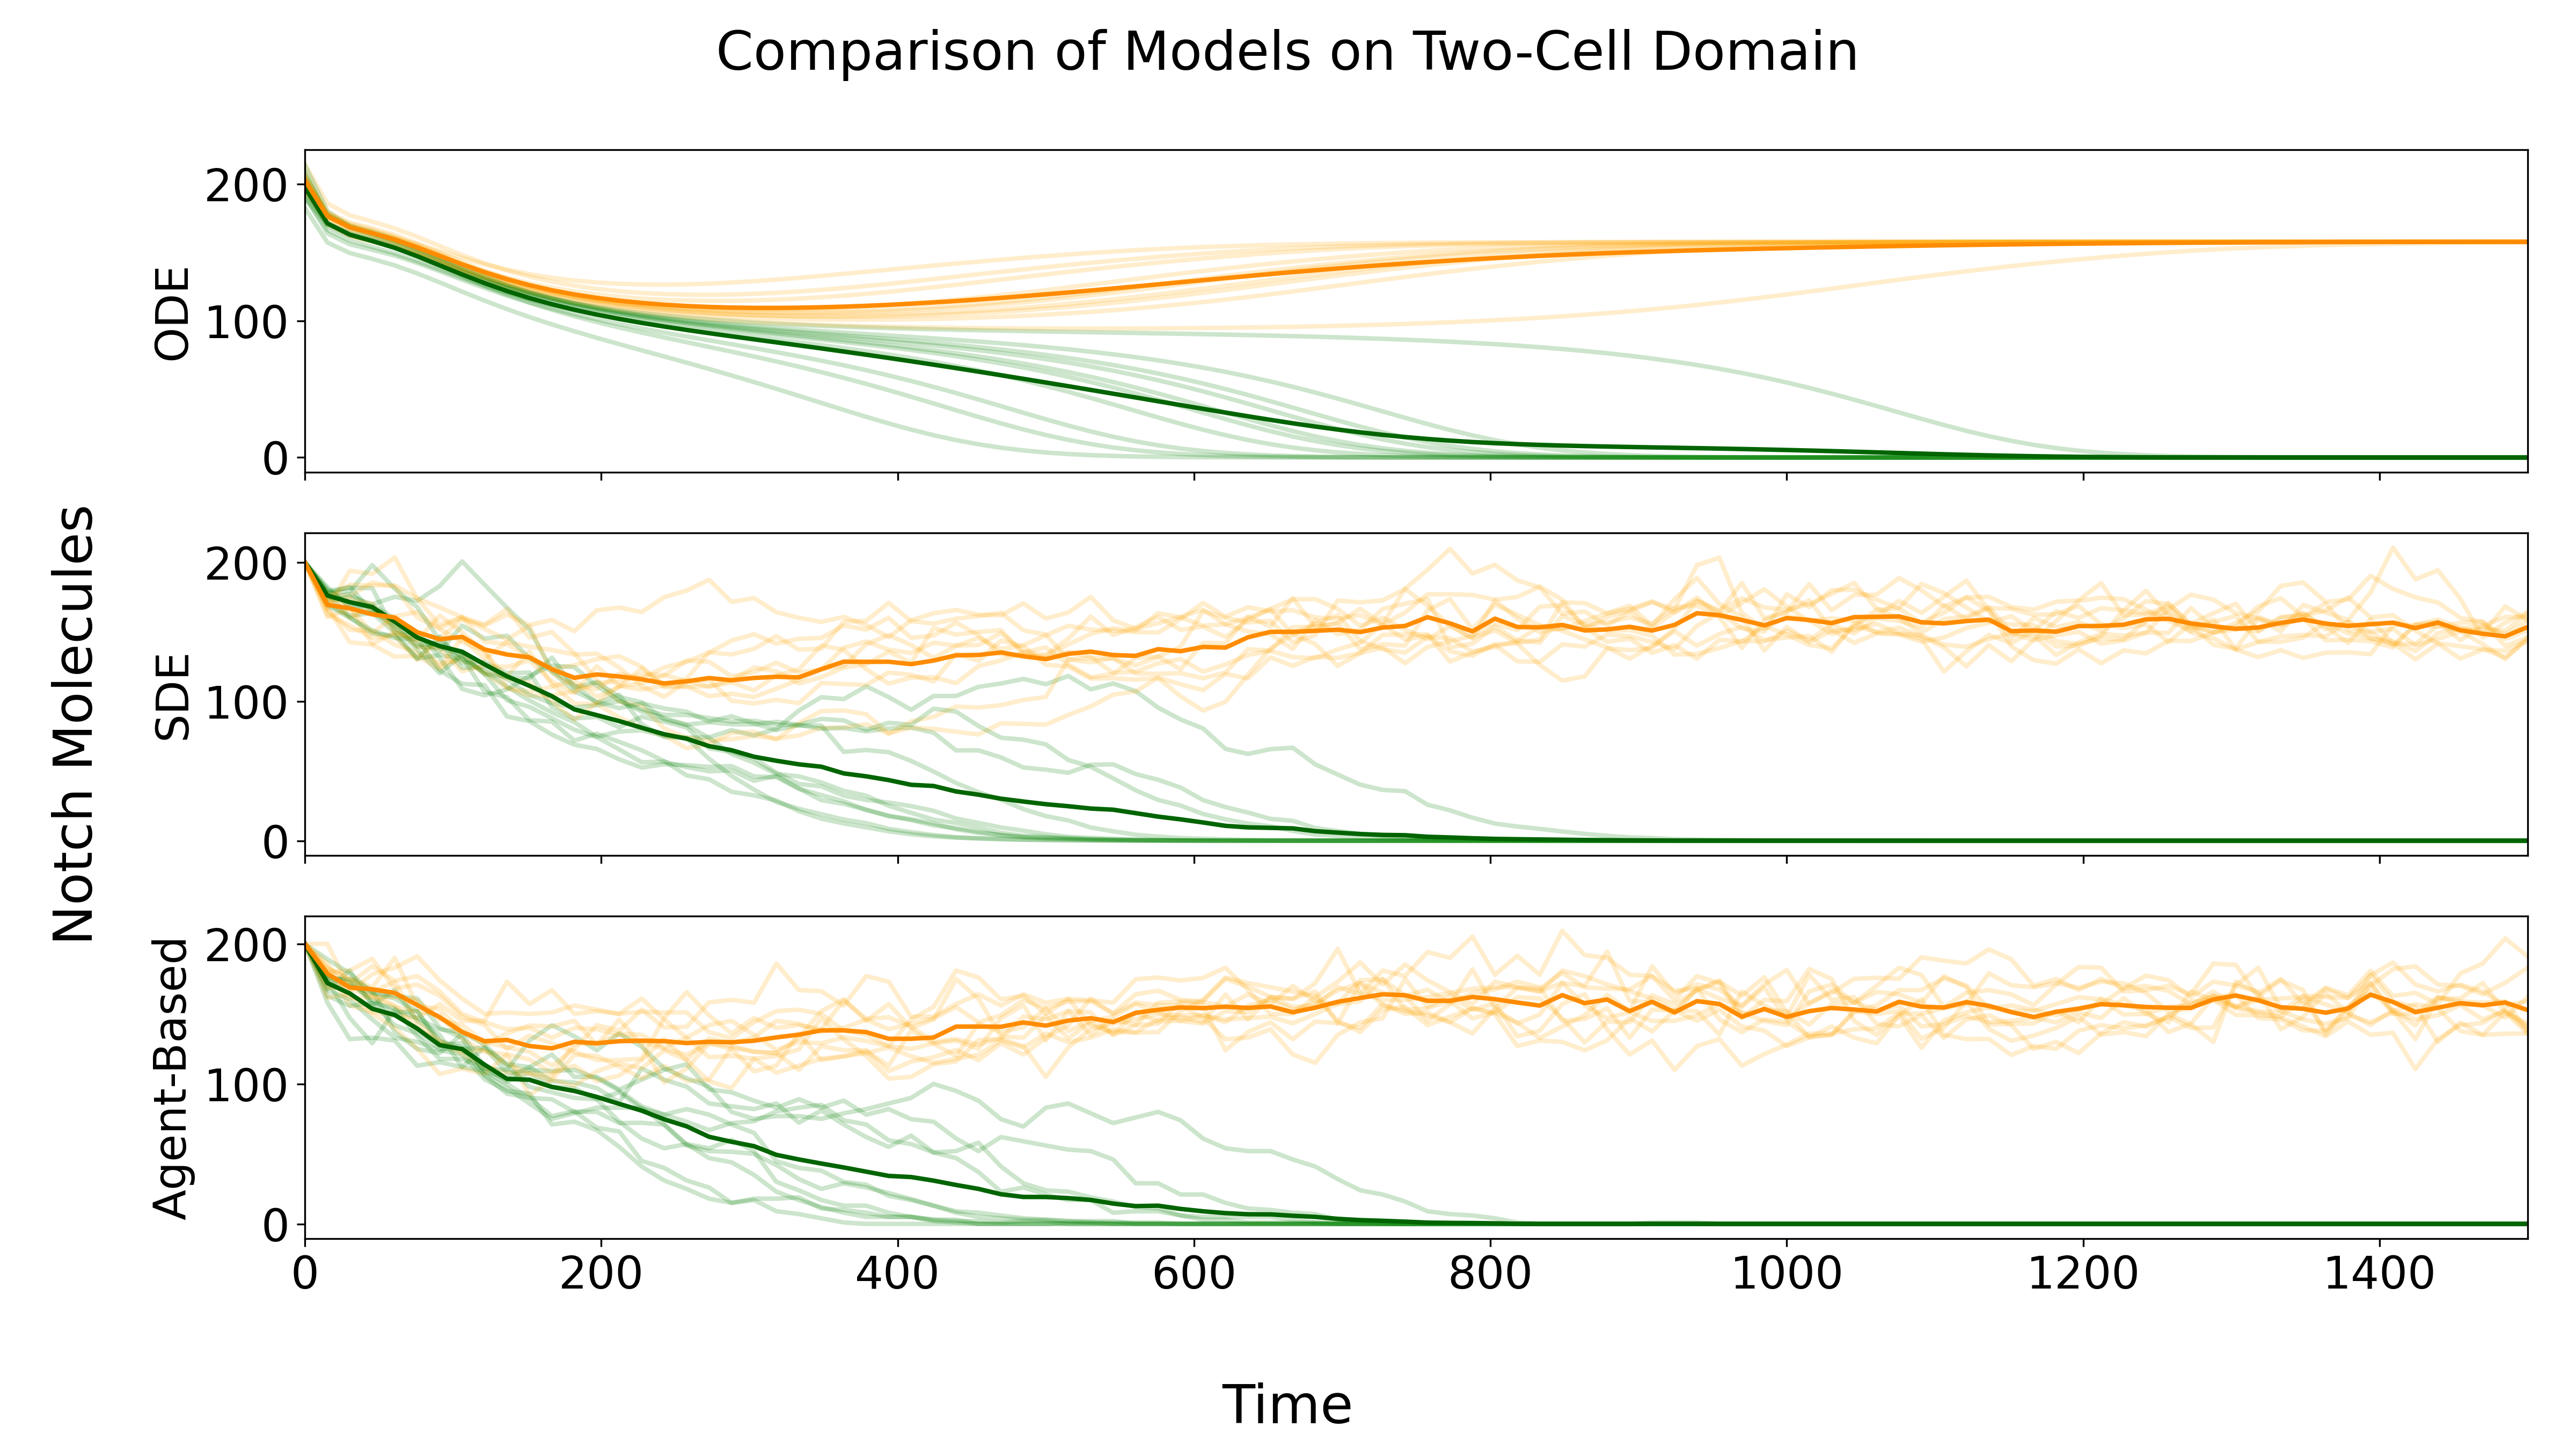
\includegraphics[width=\textwidth]{img/vis123.png}
  \caption{Results of ten simulations of each modelling formalism (ODE, SDE, agent-based) on a two-cell domain with periodic boundary conditions. An initial perturbation was applied to the ODE model to move the system off of an unstable steady state. In all simulations, the system eventually converged to a differentiated state. The number of Notch molecules in the primary-fated and secondary-fated cells  are shown in green and yellow respectively. The bold line denotes the mean number of Notch molecules over all simulations.}
  \label{fig:two-cell-simulations}
\end{figure}

Using stochastic formalisms such as the SDE and agent-based models, we can investigate more nuanced questions about the behaviour of the Delta-Notch signalling network. 
For our next experiment, we attempted to quantify how easy it would be force the two-cell system to adopt a certain outcome by perturbing the initial Notch concentration.
We predicted that the cell with the lower initial number of Notch molecules would adopt the primary (low Notch) fate, while the other cell would adopt the secondary (high Notch) fate.
While our prediction was generally true, it turns out the randomness of the agent-based model makes difficult to influence the outcome of a simulation using an initial perturbation.
The results of this experiment are shown in Figure \ref{fig:outcome-forcing}.

\begin{figure}[!htp]
  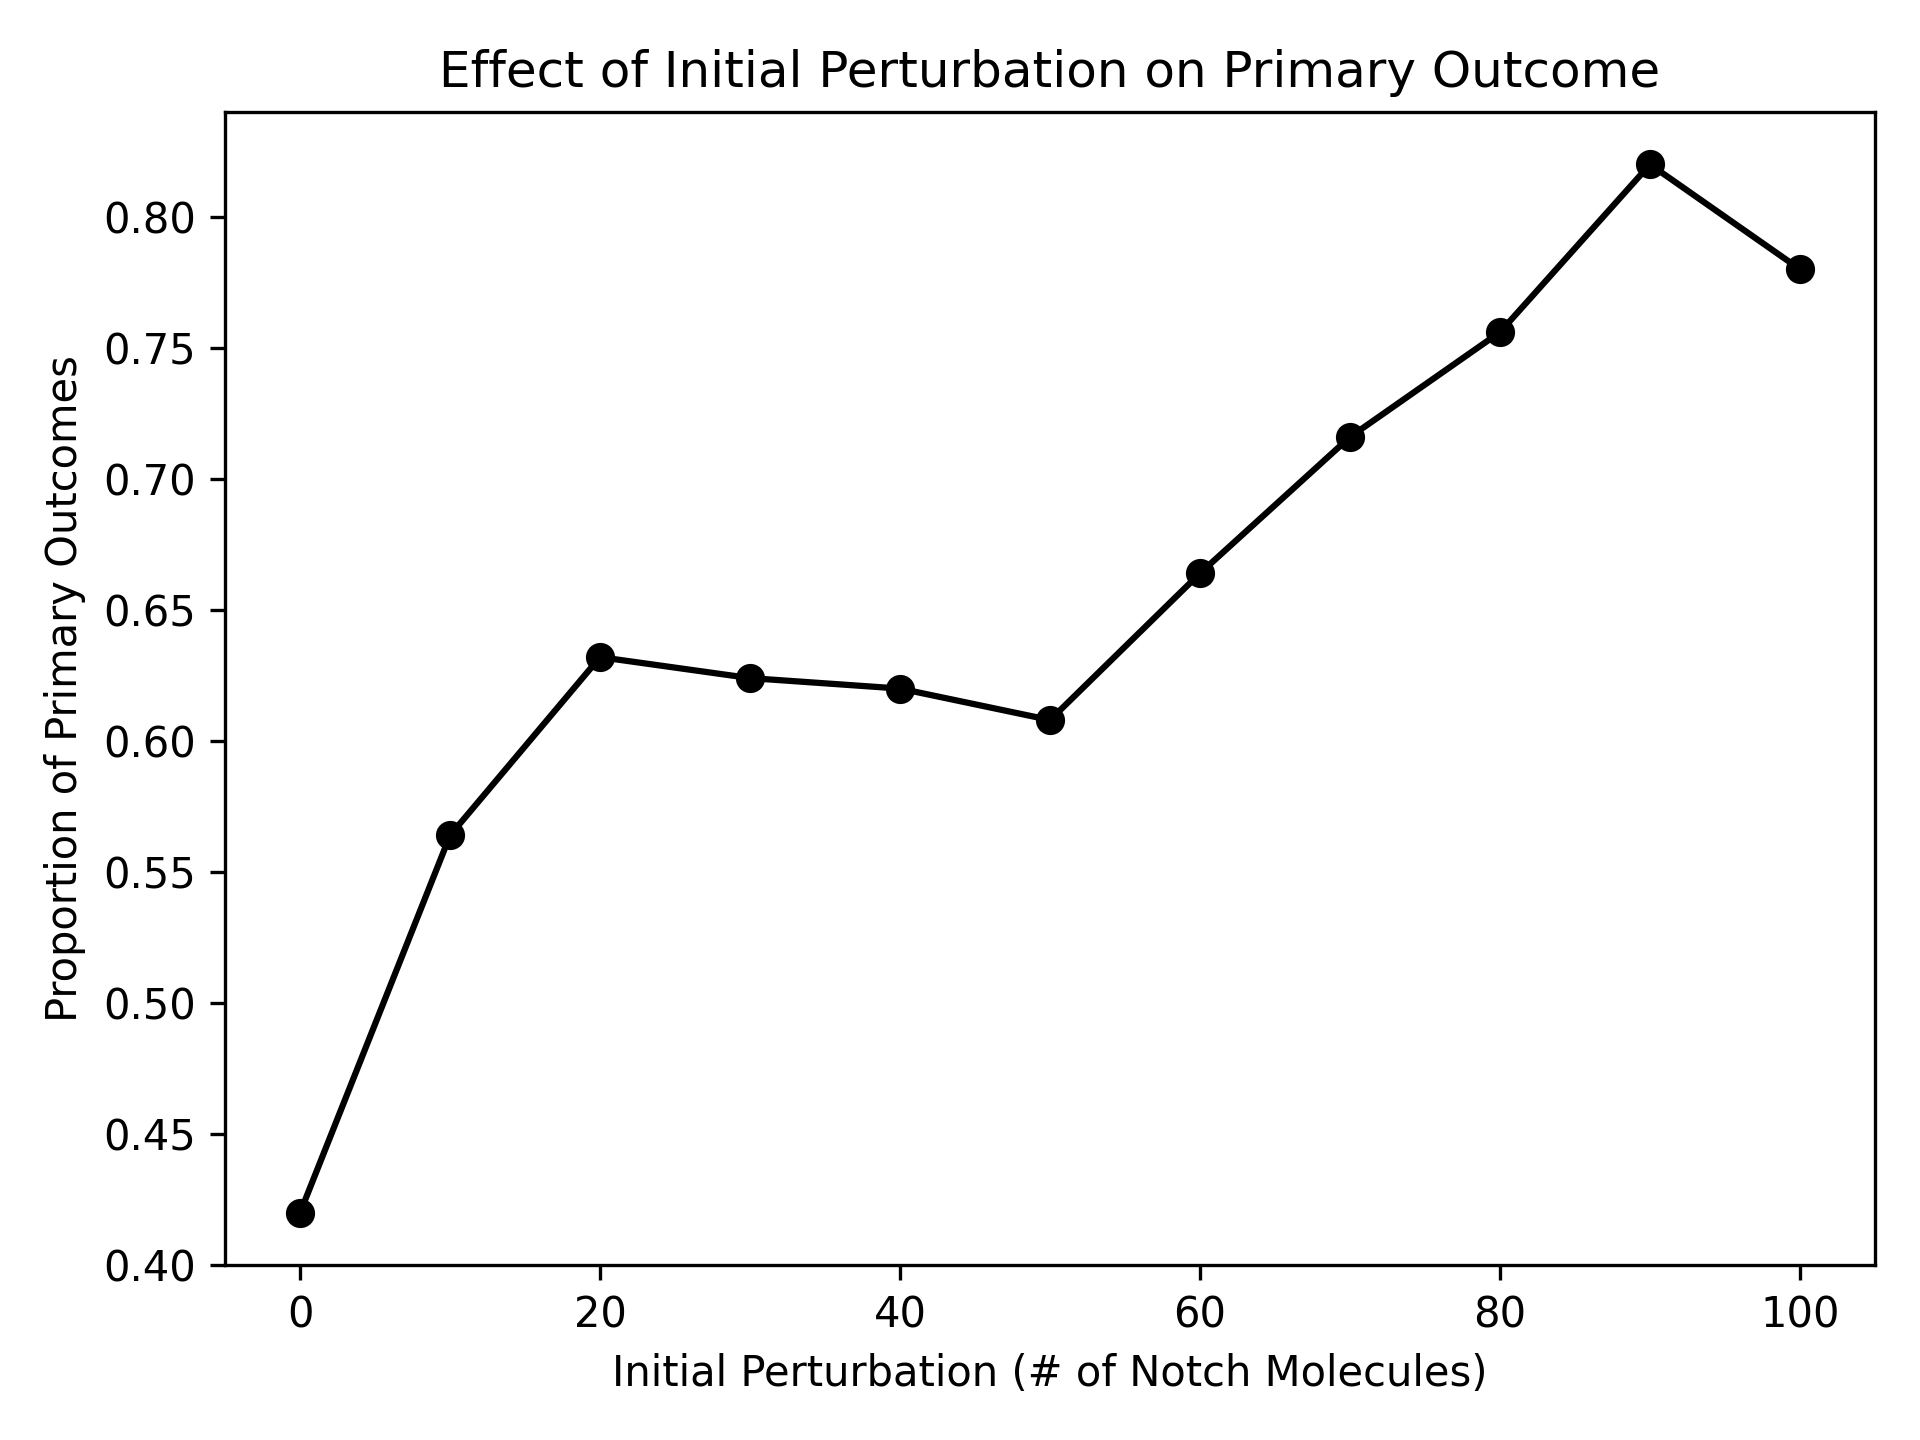
\includegraphics[width=\textwidth]{img/vis12.png}
  \caption{A \emph{Primary Outcome} occurs when the cell with the lower initial Notch concentration ends up adopting the primary (low Notch) fate. This plot shows the relationship between initial perturbation and the sample proportion of primary outcomes for the agent-based model on a two-cell domain. Prior to the perturbation, each cell has $200$ Notch molecules. A perturbation of $x$ molecules removes $x/2$ Notch molecules from the first cell and adds $x/2$ Notch molecules to the second. Unsurprisingly, larger initial perturbations result in a higher proportion of primary outcomes, although this effect is not as extreme as we expected. Even in the largest perturbation we tested ($\pm 25\%$), only $80\%$ of the simulations had the primary outcome. This suggests that it is difficult to reliably control cell fate by perturbation alone.}
  \label{fig:outcome-forcing}
\end{figure}

When we defined the SDE model in Equation \ref{eq:stochastic}, we introduced a parameter $\sigma$ that represents the amount of noise.
However, with the methods we know, it is difficult to estimate the value of this parameter analytically or numerically.
Here, we present a computational method to get an estimate of $\sigma$ which uses the differentiation time of the two-cell system.
We define the differentiation time $t^{*}$ to be the time at which one cell adopts the primary fate ($N < 1$).
Through our experiments, we noticed that higher levels of noise lower the average differentiation time by rapidly perturbing the system into more ``extreme'' states.
Using this relationship, we estimated that $\sigma = 0.02$ by comparing simulations of the SDE model with the agent-based model.
See Figure \ref{fig:noise-estimate} for a summary of this result.

\begin{figure}[!htp]
  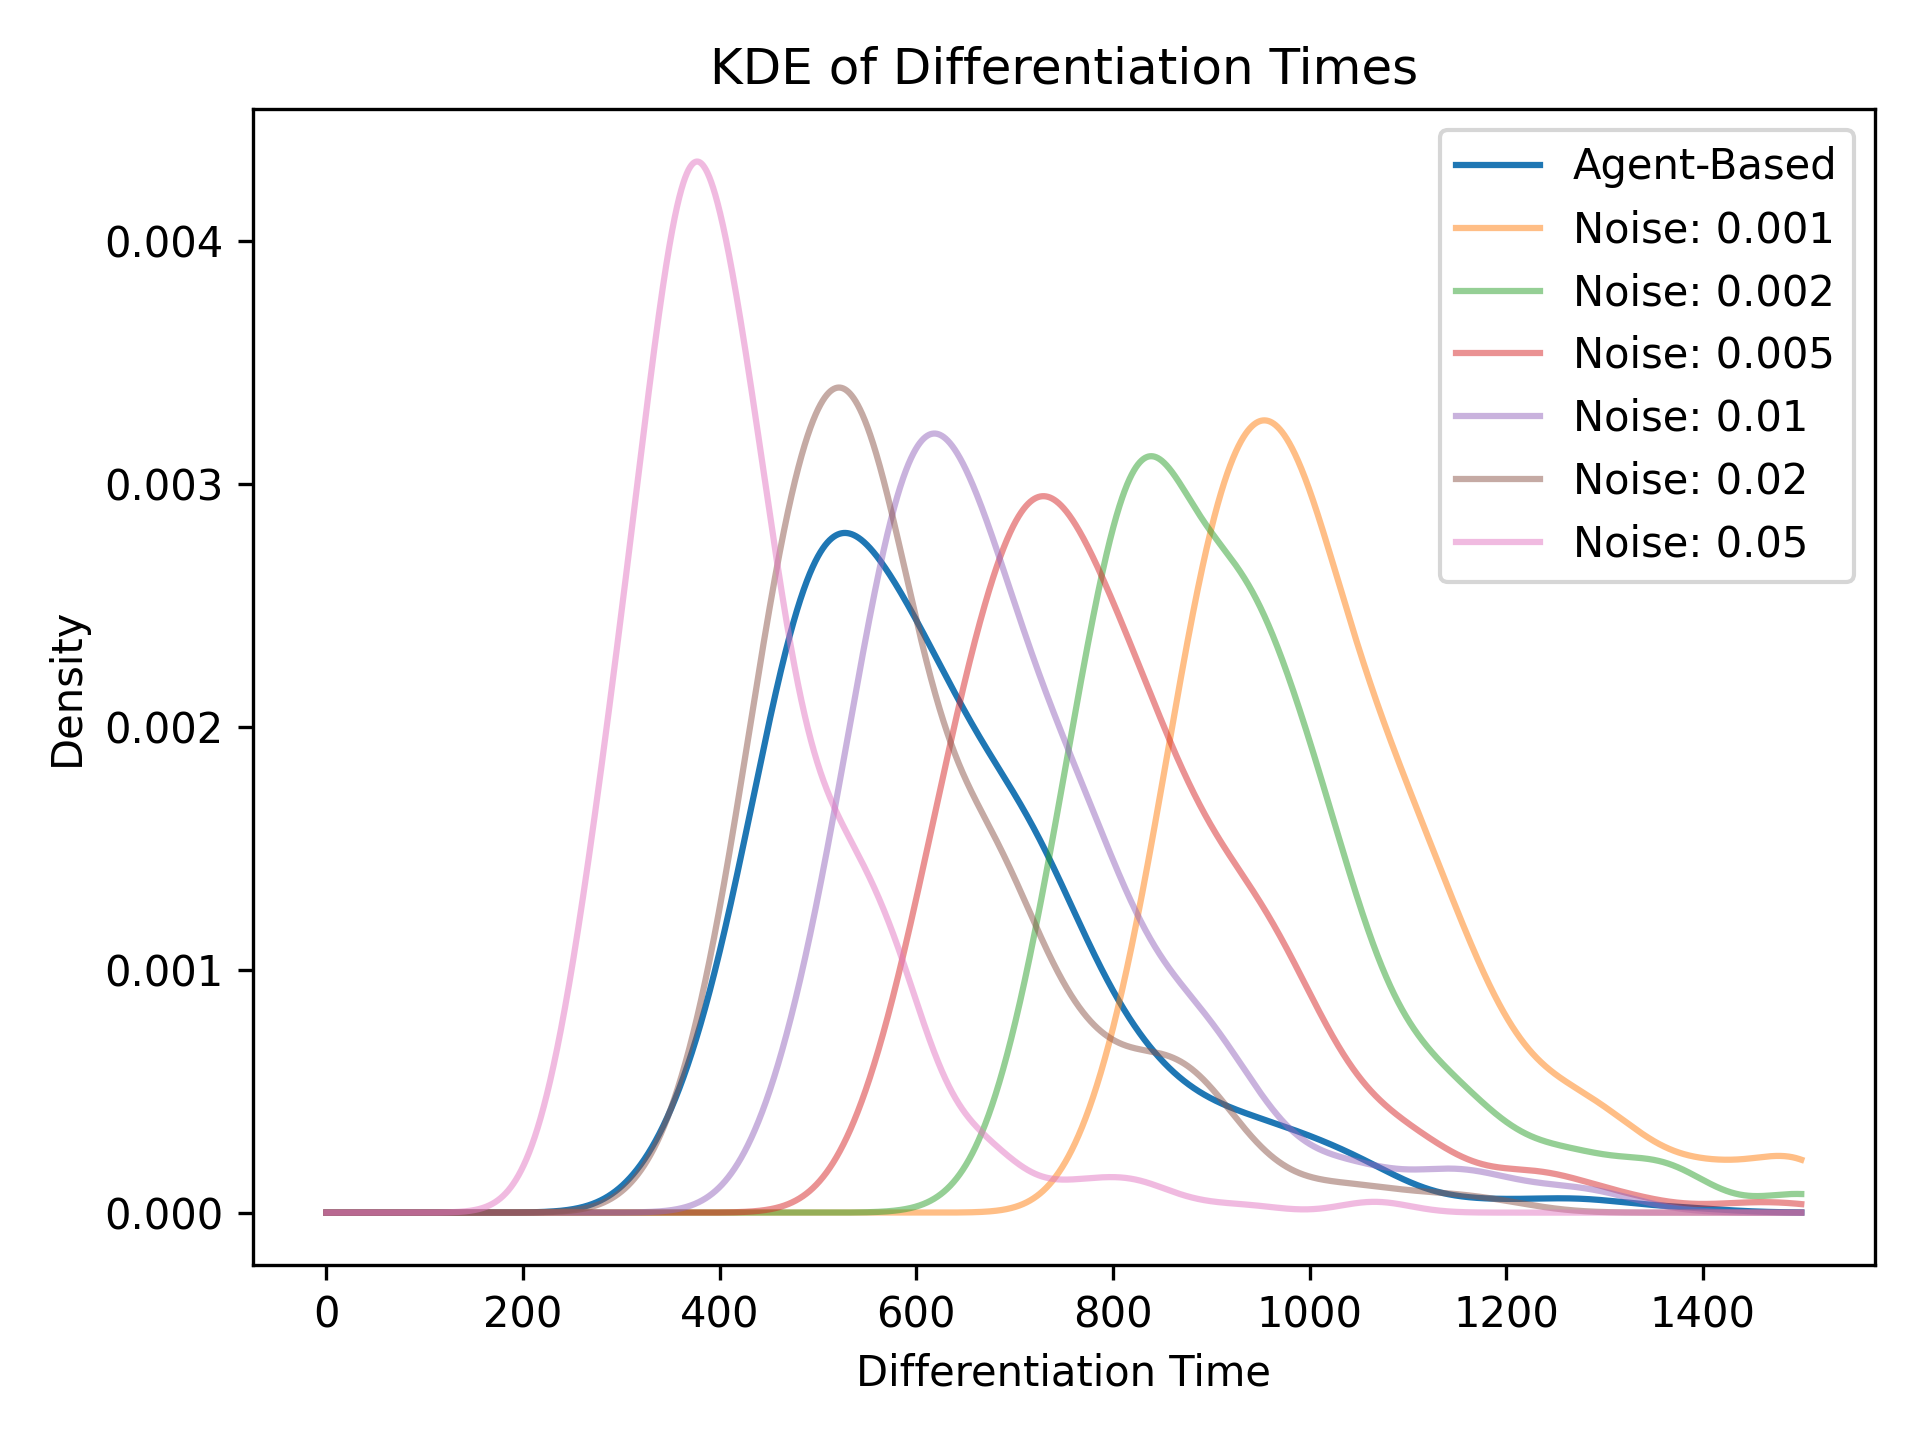
\includegraphics[width=\textwidth]{img/vis11_V2.png}
  \caption{A plot of the KDE approximation of the distribution of differentiation times for the agent-based model and the stochastic ODE model with different levels of noise. All simulations were done on a two-cell domain with periodic boundary conditions. These simulations show that higher values of the noise parameter significantly decrease the average time it takes for the two cells to adopt different fates. Notably, a noise parameter of $2\%$ causes the stochastic ODE model to align most closely with the results of agent-based simulations. }
  \label{fig:noise-estimate}
\end{figure}

All of the previous experiments were run using a fixed set of parameter values.
However, in order to evaluate the quality of our model, we wanted to see if we could replicate the key result of cell differentiation under different parameter regimes.
We identified five main parameters which determine whether the two-cell system differentiates.
These parameters are the maximum rates of Notch and Delta production $n_{m}$ and $d_{m}$, the binding rate $k_{T}$, the Notch and Delta decay rate $\gamma$, and the NICD decay rate $\gamma_{I}$.
Due to computational limitations, we could not perform a complete grid search of the $5$-dimensional parameter space.
Instead, we opted to explore all $10$ of the $2$-dimensional subspaces of our parameter space.
The results of our stability analysis are shown in Figure \ref{fig:stability-analysis}.

\begin{figure}[!htp]
   \makebox[\textwidth][c]{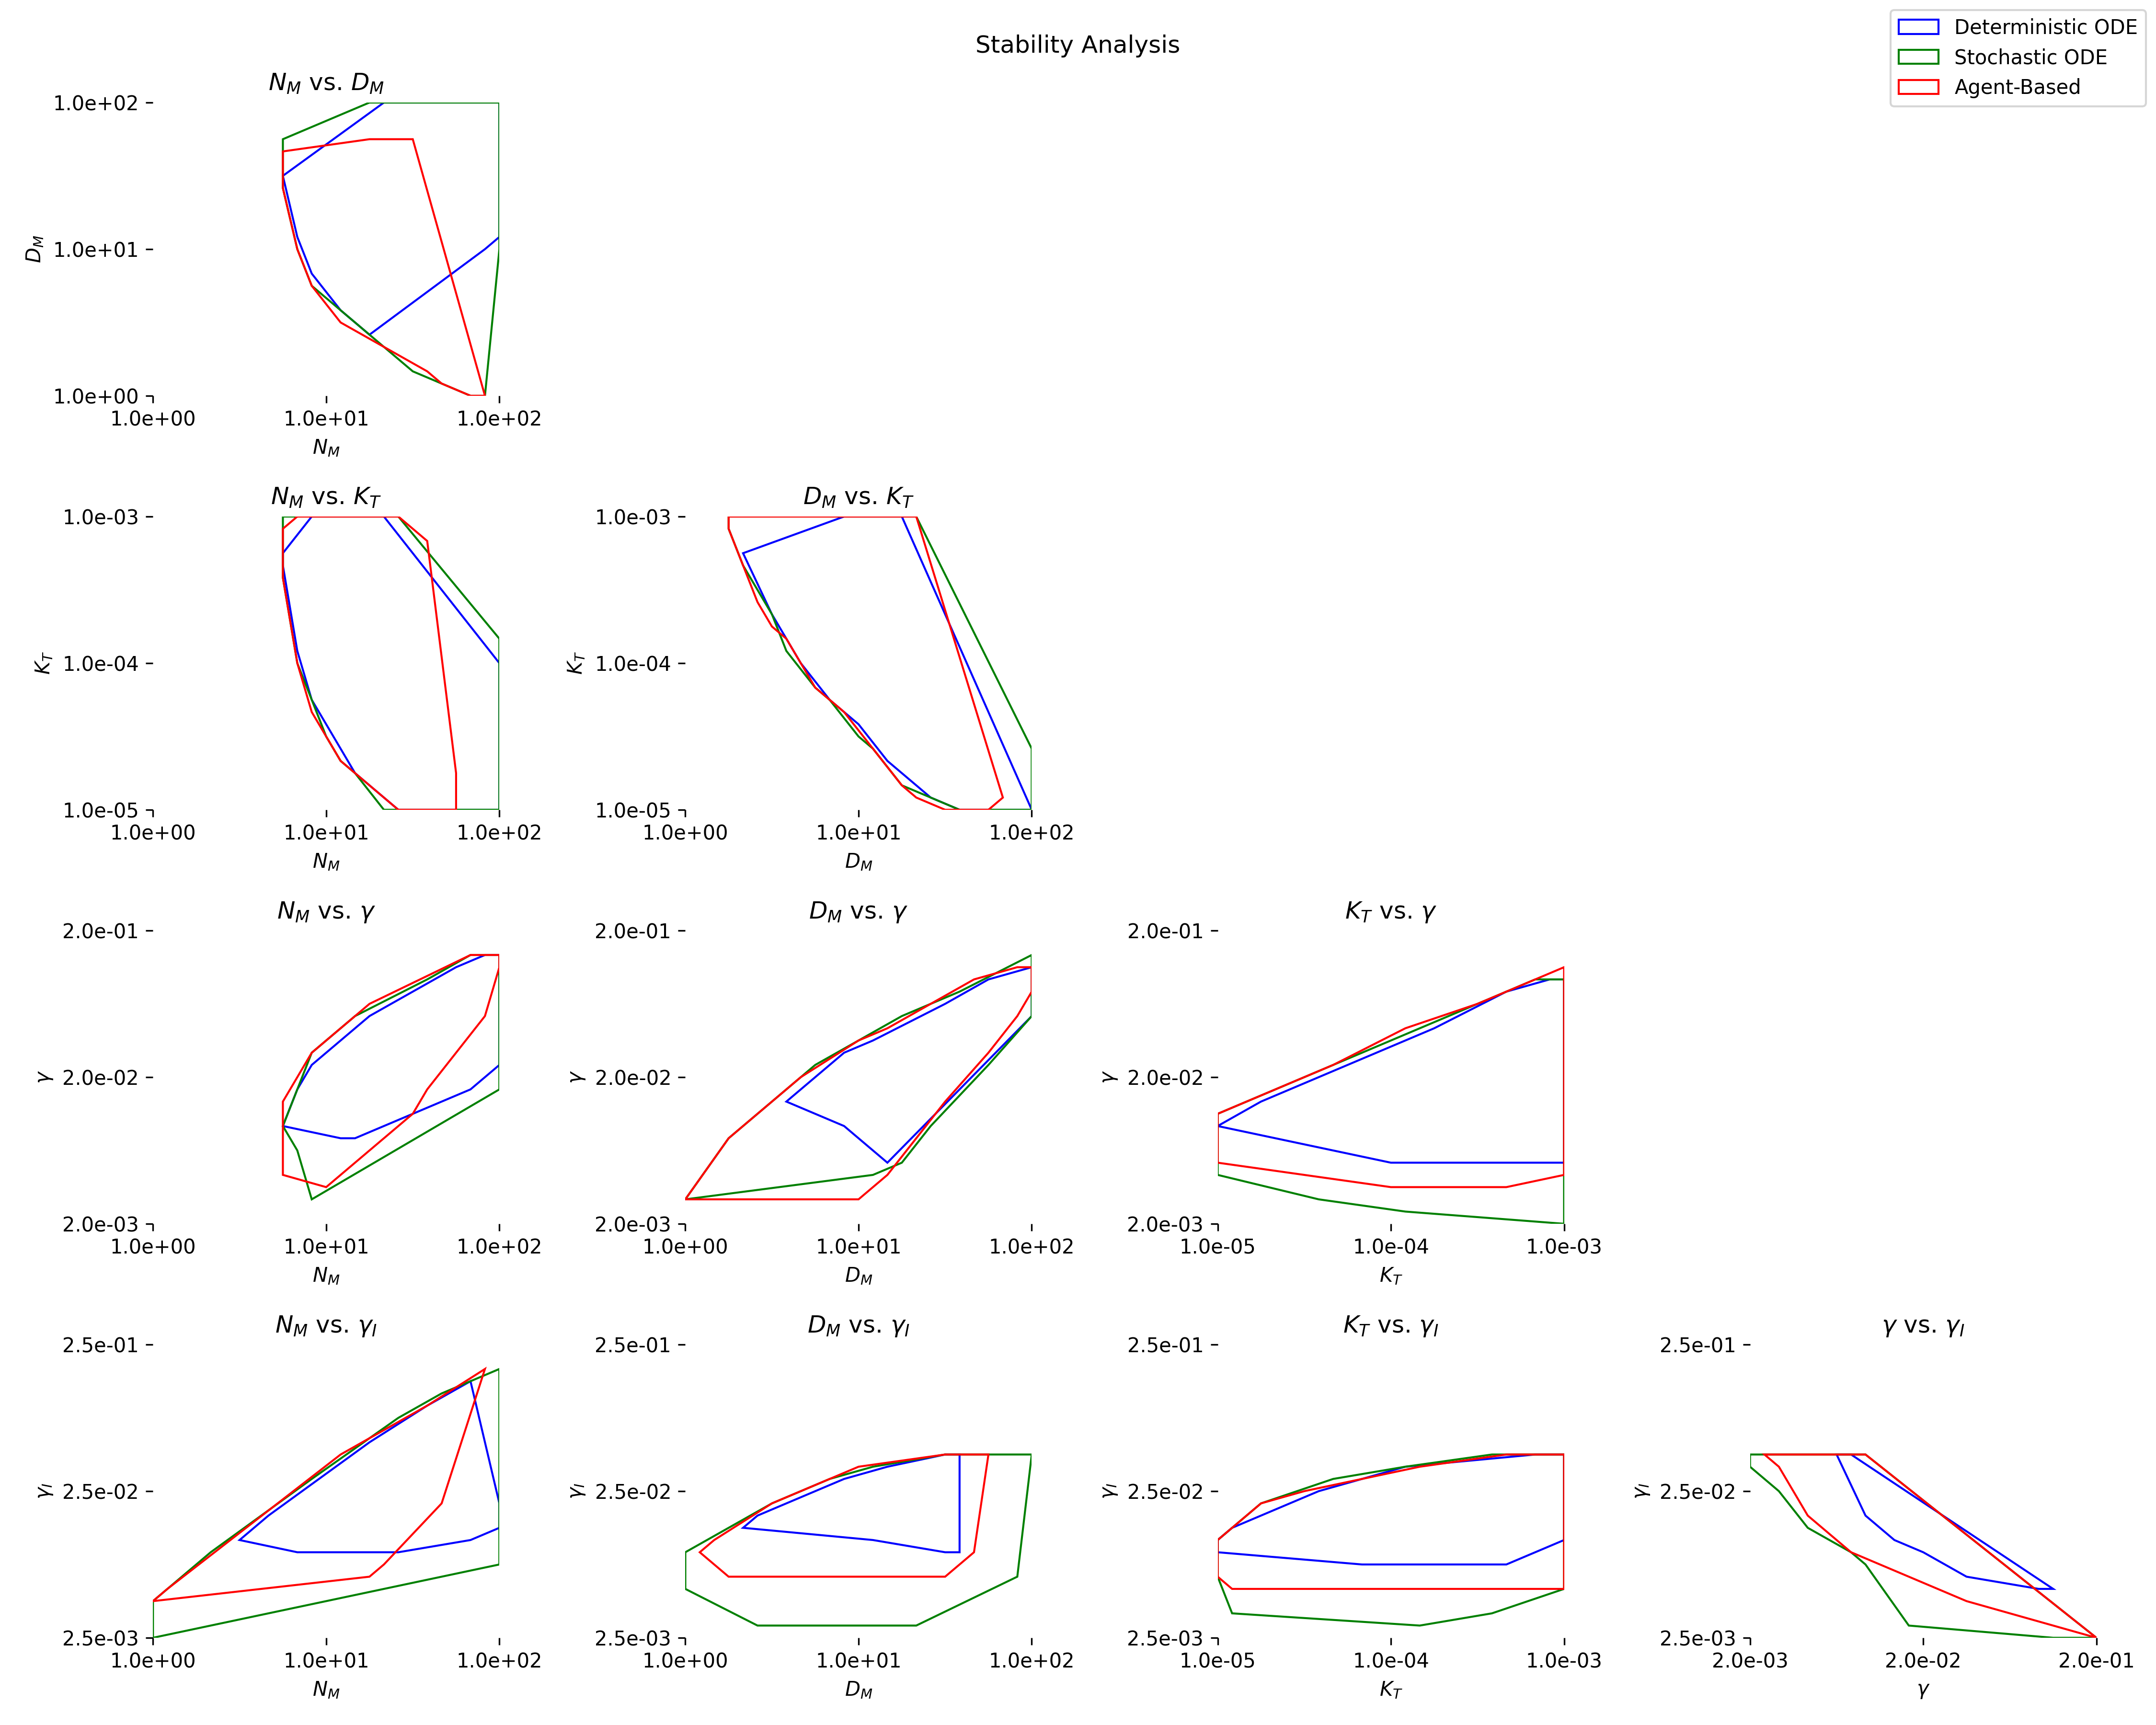
\includegraphics[width=1.3\textwidth]{img/vis13.png}}
   \caption{Results of two-at-a-time stability analysis of the deterministic, stochastic, and agent-based modelling formalisms on a two-cell domain with periodic boundary conditions. The regions enclosed by the red, blue, and green lines are regions in which cell differentiation occurs for each of the three models. Regions were obtained by simulating a $25 \times 25$ grid of test points and taking the convex hull of the points at which cell differentiation occurred. The regions are plotted with logarithmic axes. This analysis suggests that the deterministic ODE model is most sensitive to changes in the parameter regime, especially changes to $\gamma$ and $\gamma_{I}$.} 
   \label{fig:stability-analysis}
\end{figure}

\subsection*{Linear Domains}

Collier et al. \cite{collier_pattern_1996} tested their model on linear domains of up to $40$ cells with zero-flux boundary conditions.
They observed that cells on the boundary of the domain adopted a fate first.
Then, the alternating pattern of primary and secondary fated cells gradually spread inwards towards the center of the domain.
In our first experiment on a linear domain, we replicated this result as shown in Figure \ref{fig:linear-domain}. 

\begin{figure}[!htp]
   \makebox[\textwidth][c]{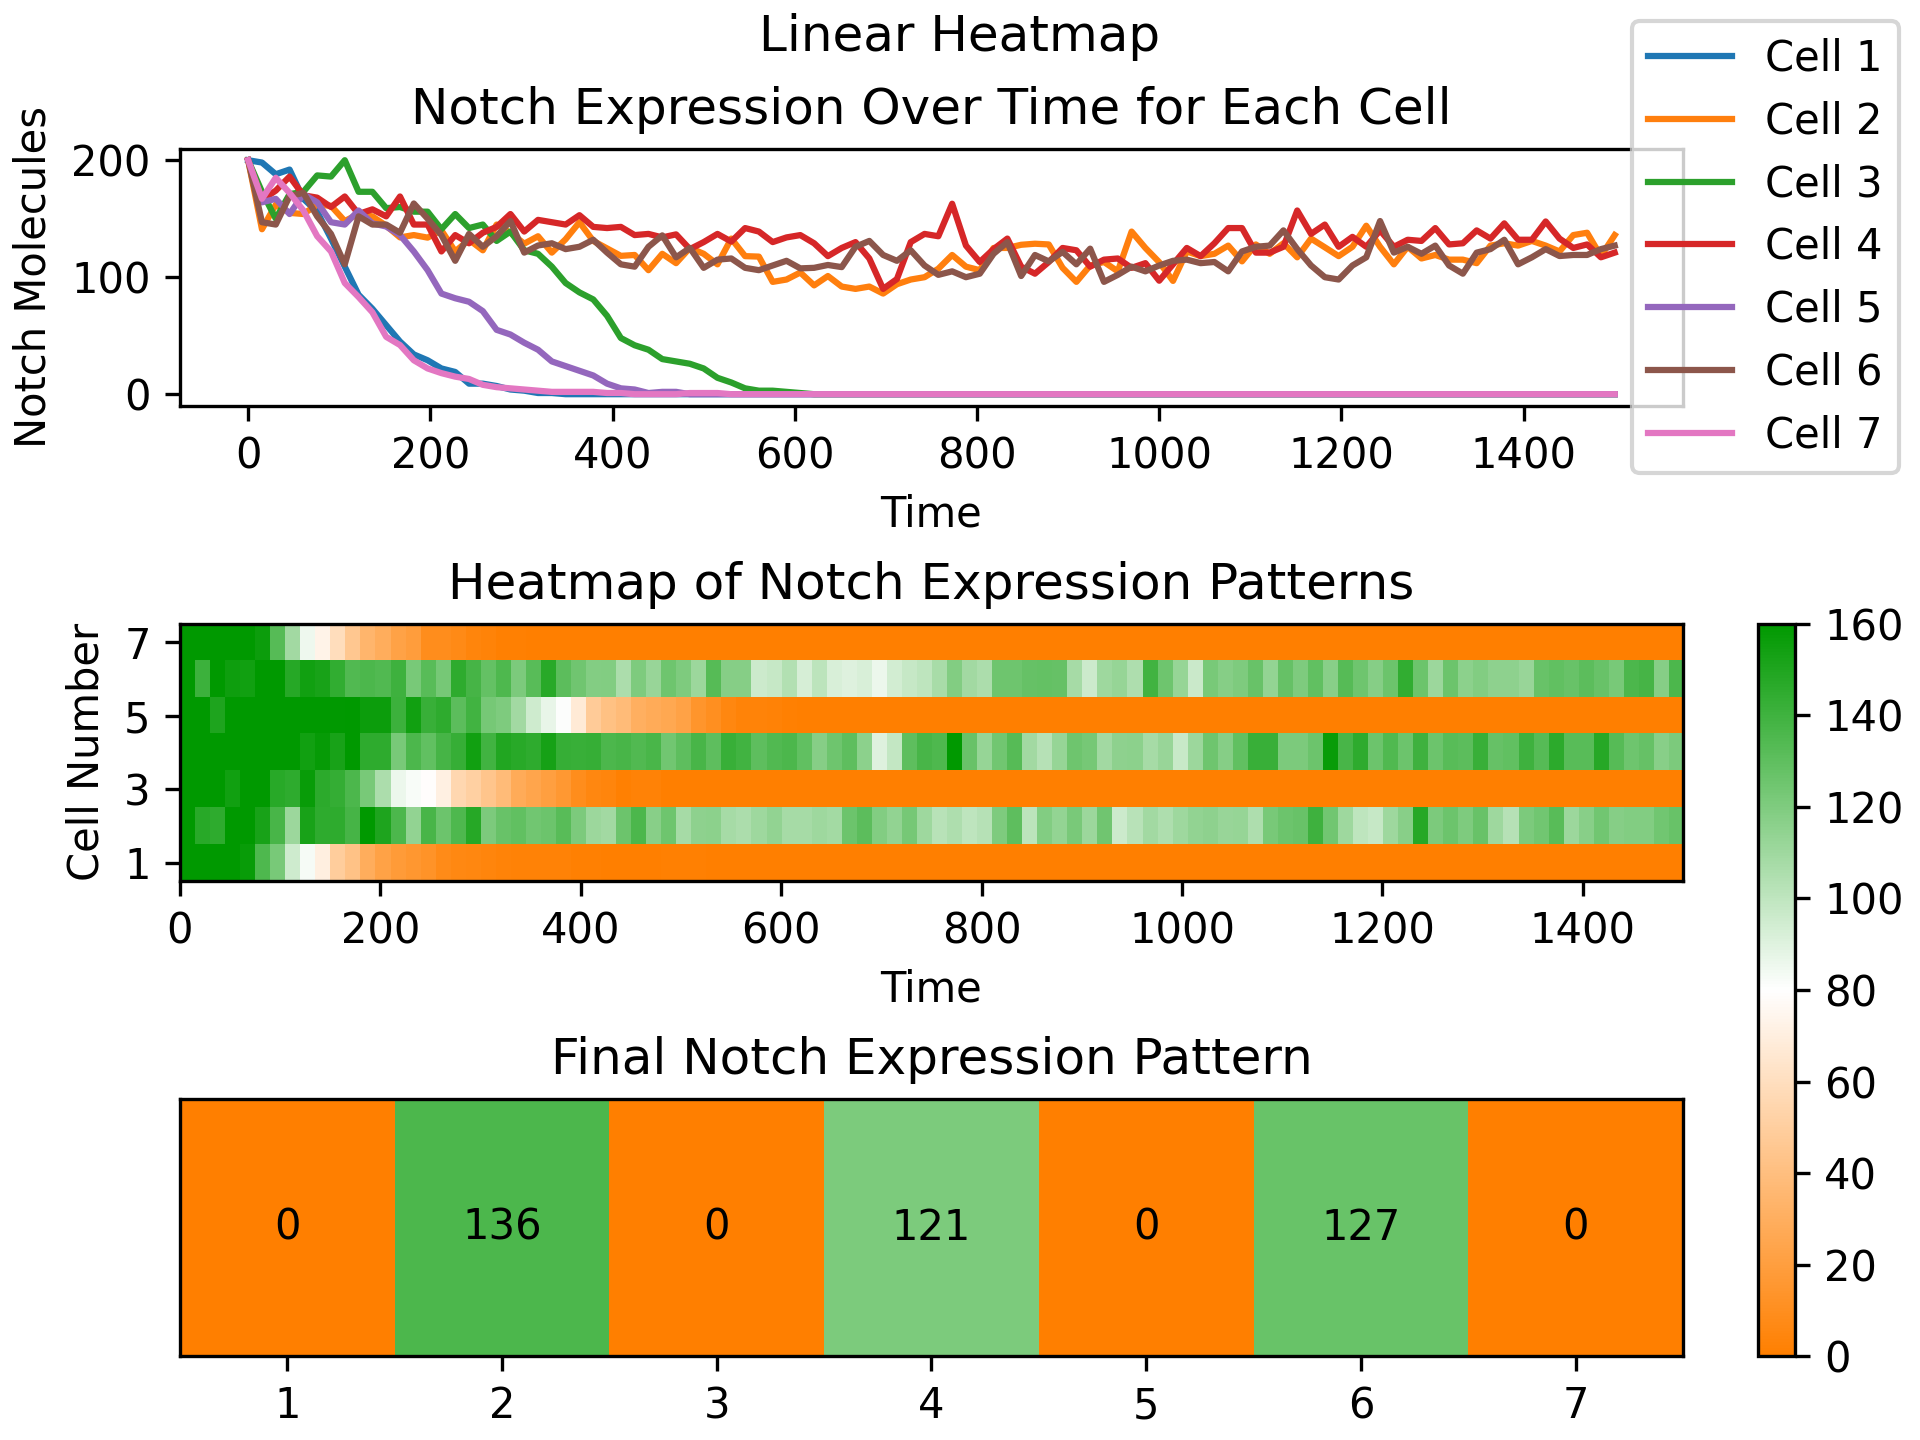
\includegraphics[width=1.3\textwidth]{img/linear_heatmap_Gillespie_V1.png}}
   \caption{
Results of the agent-based model run on a linear domain with 7 cells using Dirichlet boundary conditions.
The first subplot shows Notch molecules per cell over time.
Since noise is introduced every time step, the cell trajectories exhibit Brownian motion-like behaviour and thus have been smoothed out for better legibility.
The second plot also shows Notch levels over time but in this visualization it is easier to see how cells influence their neighbours and how the cells on the edge of the domain are first to differentiate.
The third plot shows the final Notch pattern, where primary fate cells are orange (indicating low Notch) and secondary fate cells are green (indicating high Notch).} 
   \label{fig:linear-domain}
\end{figure}

We also attempted to broadly classify the types of patterns we observed on linear domains.
In order to do this, we needed to define the notion of a \emph{pattern}.
Since the ``default'' outcome of a simulation on a linear domain is an alternating array of cells with each fate, we will call this pattern $0: [],\, 1: []$.
Then, each contiguous group of cells with the same fate (where $0$ is the primary fate and $1$ is the secondary fate) will add entries to the pattern arrays.
For example, if there are $2$ contiguous pairs of cells with the primary fate and $1$ contiguous triplet of cells with the secondary fate, the simulation will have the pattern $0: [2, 2], \, 1: [3]$. 
There is a lot more nuance related to pattern formation that we were unable to explore, but one interesting result is shown in Table \ref{tb:patterns}.

\begin{table}[!htp]
\centering
\begin{tabular}{|c|c|c|c|} 
 \hline
 Pattern & Frequency (Odd Domain) & Frequency (Even Domain)  \\
 \hline
 $0: [], \, 1: []$ & $87$ & $403$ \\
 $0: [], \, 1: [2]$ & $801$ & $123$ \\
 $0: [], \, 1: [2, 2]$ & $27$ & $424$ \\
 $0: [], \, 1: [2, 2, 2]$ & $48$ & $1$ \\
 \hline
\end{tabular}
\caption{
  Frequency of selected cell patterns in $1000$ simulations of the agent-based model on $9$-cell (even) and $10$-cell (odd) domains with zero-flux boundary conditions.
  We observe significant variations in patterns across even and odd domains.
  Similarly drastic variation is observed across different modelling formalisms and boundary conditions (not shown).
}
\label{tb:patterns}
\end{table}

Another phenomenon that we discovered, although we did not explore in detail, is that the SDE model was far more likely to allow for adjacent pairs of primary fate cells than the agent-based model when given identical parameter values and initial conditions.
The agent-based model showed greater robustness to parameter change than the SDE model, as the general differentiation pattern noted by Collier et al. (shown in Figure \ref{fig:linear-domain}) could easily be disrupted by small adjustments to the binding coefficient $k_T$ or the Notch/Delta decay rate $\gamma$ leading to primary fate cell grouping.

\subsection*{Hexagonal Domains}

Continuing to use the domains in Collier et al. \cite{collier_pattern_1996}, we next considered hexagonal grids of cells in a slanted parallelogram pattern. 
We imposed both periodic and Dirichlet boundary conditions on these grids.
In our simulations, we observed alternating patterns of primary fate cells appear on the $7$x$7$ grid (see Figure \ref{fig:hexagonal-domain}), especially for the agent-based model.
Although the SDE model could replicate this same pattern depending on initial conditions, it was more likely to end up with pairs of adjacent low-notch cells.
This behaviour was not noted by Collier et al. and points to some key differences between our models depending on the domain.

\begin{figure}[!htp]
   \makebox[\textwidth][c]{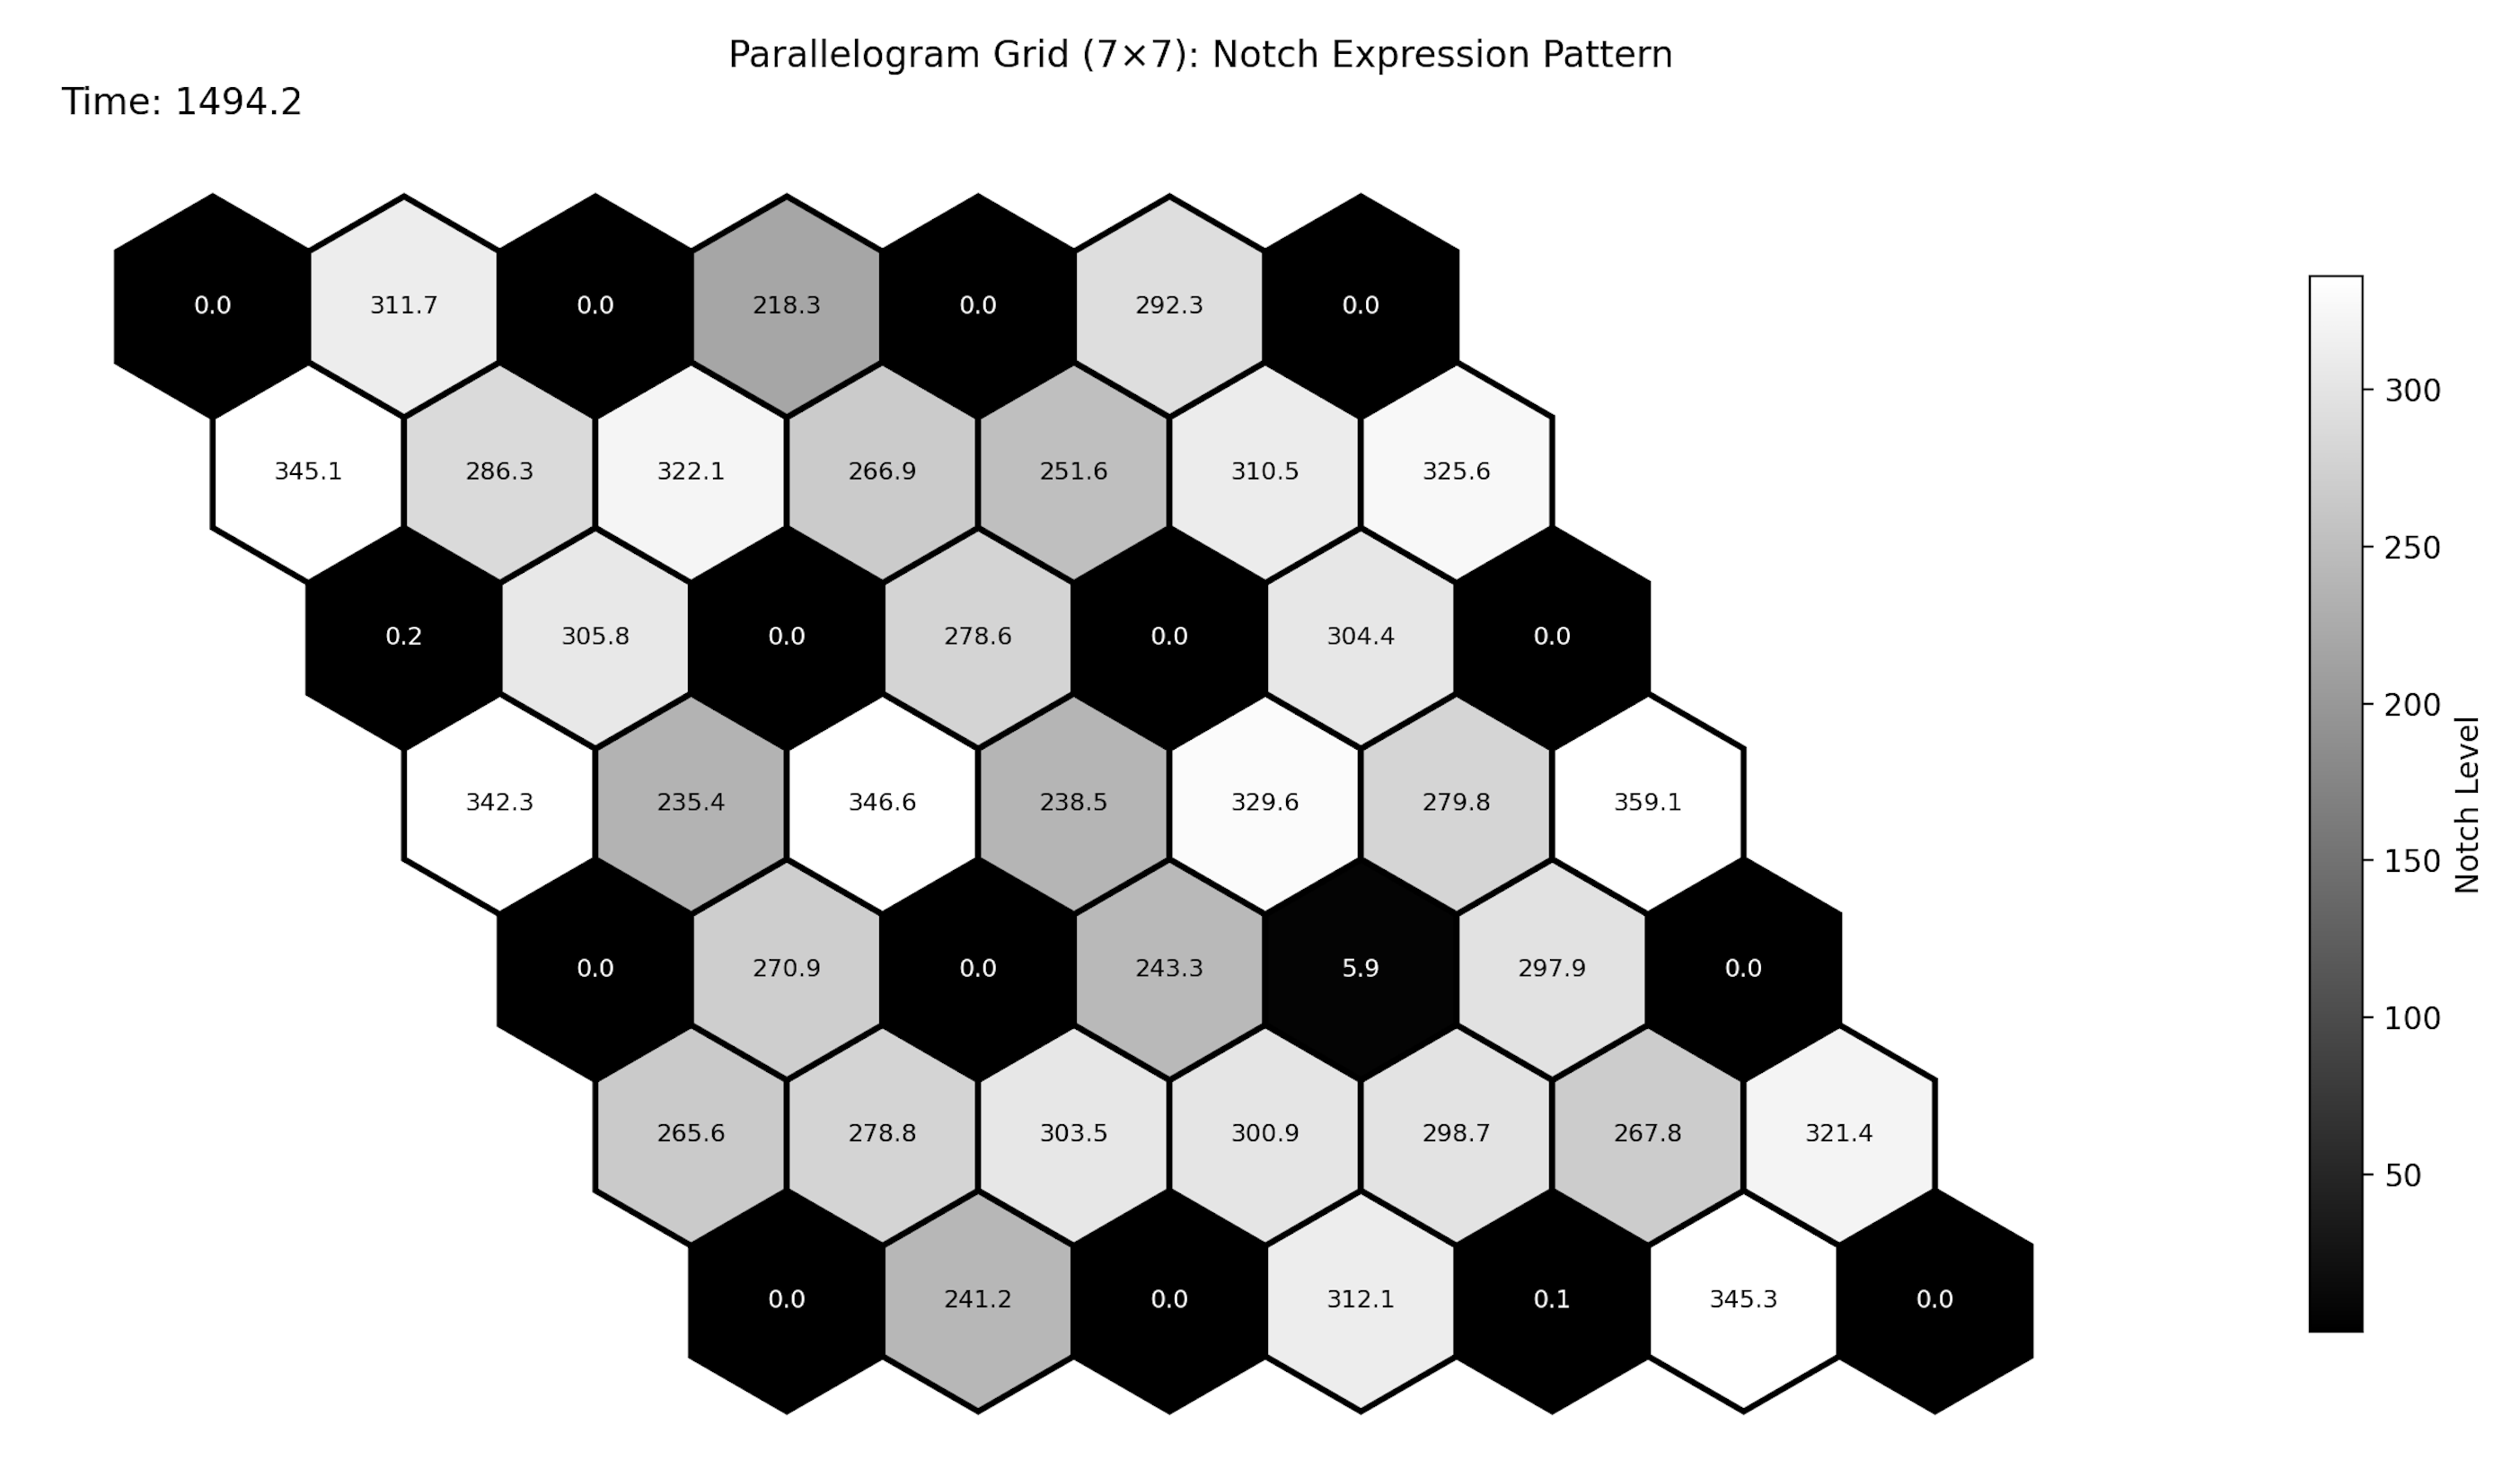
\includegraphics[width=1.3\textwidth]{img/HexDirichletPattern.png}}
   \caption{Results of the agent-based model run on a hexagonal domain with 49 cells using Dirichlet boundary conditions. In this figure, black represents primary cell fate and white secondary cell fate. Although not all the secondary fated cells have the same Notch levels, this general pattern is stable long term with high Notch concentration around $300$ molecules.} 
   \label{fig:hexagonal-domain}
\end{figure}

The patterns on the hexagonal domains also exhibited increased sensitivity to boundary conditions and parameter values.
In particular, identical starting conditions and parameters would often lead to markedly different final patterns on domains with periodic and Dirichlet boundary conditions.
Figure \ref{fig:hexagonal-compare} highlights some of these differences.
Increasing $\gamma$ from $0$ to $0.03$ could leave final patterns showing homogeneous cell fate, isolated primary cells, or even striping behaviour.
Similar to the linear domain, cells on the edge of the hexagonal domain tended to differentiate first, especially when using Dirichlet boundary conditions.

\begin{figure}[!htp]
   \makebox[\textwidth][c]{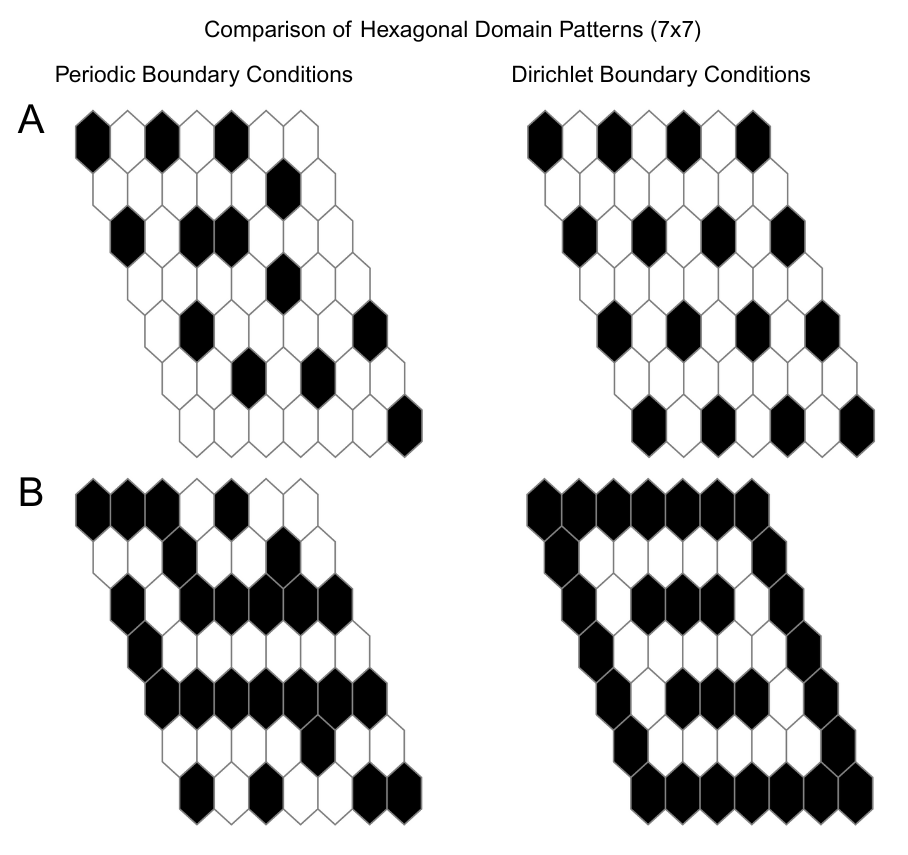
\includegraphics[width=1.3\textwidth]{img/Hex_Compare.png}}
   \caption{Results of running the SDE model on 49 hexagonal cells, with identical initial conditions comparing periodic and Dirichlet boundary conditions. Cells are coloured black if the notch level is less than $1$ at the final time step and left white otherwise. The first row (A) uses $\gamma = 0.01$ while the second row (B) uses $\gamma = 0.02$. All other parameters are equal for these simulations. }
   \label{fig:hexagonal-compare}
\end{figure}

\section*{Discussion}

Our comparison of the ODE, SDE, and agent-based models highlights a clear trade-off between simplicity and accuracy in modelling Delta-Notch signalling.
The ODE model is computationally efficient and easy to analyze, but can only break symmetry with an initial perturbation.
In other words, stable cell differentiation only occurs when the initial conditions are already imbalanced.
Under the SDE model, the additional noise allows cells to break symmetry without perturbations.
This behaviour closely mirrors the agent-based model, which captures randomness at the level of individual molecules.
Although cell differentiation was easy to achieve with the stochastic models, controlling cell fate proved to be more challenging than we initially expected.
Even when we imposed large initial perturbations in the two-cell system ($\pm 25\%$), the intended outcome only occurred about $80\%$ of the time.
This result suggests that there are systemic biases in the Delta-Notch signalling pathway that induce specific fates in certain cells. 


When comparing the SDE model to the agent-based model, we found that the differentiation time varied considerably depending on the noise coefficient $\sigma$.
To ensure these two models produced consistent results, we carefully tuned the noise coefficient to an optimal value of $\sigma = 0.02$.
Finally, we concluded our investigation of the two-cell domain with a stability analysis, which found that the ODE model is the most sensitive to changes in parameter values, especially the decay rates $\gamma$ and $\gamma_{I}$.
On linear domains, all three models exhibited the behaviour described by Collier et al., with an approximately alternating pattern of cell differentiation spreading inward from the edges.
However, the SDE model and the agent-based model deviated from perfect alternation in the majority of simulations.
Furthermore, the deviations were different between the two models, as contiguous groups of primary fated cells almost never appeared in agent-based simulations but appeared frequently in simulations of the SDE model.
This variability points to a key biological insight: while randomness provides flexibility and diversity in pattern formation, it can also make patterns less predictable, particularly in small systems or near critical parameter boundaries.

Finally, we replicated the qualitative results of Collier et al. on two-dimensional hexagonal domains. 
We also found that our models were more sensitive to changes in parameter values and boundary conditions on the hexagonal domain compared to the linear and two-cell domains.
However, due to computational limitations and time constraints we were unable to do a more thorough analysis of the models' behaviour on the hexagonal domain.
Generally, our results on all three domains show that the choice of modelling formalism can drastically influence the results of simulations.
Therefore, we suggest that modellers should also investigate whether their results are stable across different formalisms (a ``model stability analysis'') whenever possible.

\nocite{*}
\printbibliography

\appendix

\begin{flushleft}

\section{Gillespie's Algorithm} \label{sec:gillespie}

Gillespie's algorithm allows us to simulate many types reactions simultaneously using random time steps. Recall that $T_{i}$ is a random variable that represents the distribution of the next reaction of any type. The random variables $X_{1}, \dots, X_{N}$ are the waiting time distributions for each reaction $1, \dots, N$, where $N = (6 \times \text{\# Cells})$.

\textbf{Step 1}: Sample a value $t_{i}$ from $T$ using inverse transform sampling. 

\textbf{Step 2}: Increment the current time $t$ by $t_{i}$.

\textbf{Step 3}: Determine which event took place. To do this, recall that:

$$P(X_{k} = \text{min} \{  X_{1}, \dots, X_{N} \}) = \frac{\lambda_{k}}{\lambda_{1} + \dots + \lambda_{N}}$$

Use this fact to partition the interval $[0, 1]$. Then sample $y_{i}$ from a $\text{Unif}(0, 1)$ distribution, identify its partition, and find the corresponding event.

\textbf{Step 4}: Update the state based on the event determined in the previous step.

\textbf{Remark}: The expected time for reaction $i$ to occur is given by $\mathbb{E}[X_{i}] = 1/\lambda_{i}$. Therefore, the rate at which event $i$ occurs is $\lambda_{i}$, which is equal to the rate at which the event occurs in the original ODE. This means that the trajectories generated from the Gillespie's algorithm implementation of the agent-based  model can be compared directly to the trajectories generated from the ODE itself, without any need for scaling.


\section{Kolmogorov Forward Equations}
\label{sec:kfe}


\subsection*{Derivation of Kolmogorov Forward Equation}
For simplicity, we consider the dynamics of a single cell (cell $A$) in the following derivations.

Let us define:
\begin{itemize}
    \item $P(n,d,i,t)$: the probability of having $n$ Notch receptors, $d$ Delta ligands, and $i$ NICD molecules in cell $A$ at time $t$.
    \item $D_{ext}$: the average number of Delta molecules in the neighbourhood of cell $A$.
\end{itemize}

The Kolmogorov forward equation describes how $P(n,d,i,t)$ changes over a small time step $\Delta t$:
\begin{align*}
P(n,d,i,t+\Delta t) &= P(n,d,i,t) \\
&+ P(n-1,d,i,t) \cdot H^+(i) \Delta t \quad \text{(Notch production)} \\
&+ P(n,d-1,i,t) \cdot H^-(i) \Delta t \quad \text{(Delta production)} \\
&+ P(n+1,d,i,t) \cdot \gamma(n+1)\Delta t \quad \text{(Notch decay)} \\
&+ P(n,d+1,i,t) \cdot \gamma(d+1)\Delta t \quad \text{(Delta decay)} \\
&+ P(n,d,i+1,t) \cdot \gamma_I(i+1)\Delta t \quad \text{(NICD decay)} \\
&+ P(n+1,d,i-1,t) \cdot k_T(n+1)D_{ext}\Delta t \quad \text{(Trans-activation)} \\
&- P(n,d,i,t) \cdot [H^+(i) + H^-(i) + \gamma n + \gamma d + \gamma_I i + k_T n D_{ext}]\Delta t
\end{align*}

Rearranging to find the time derivative and taking the limit as $\Delta t \rightarrow 0$:
\begin{align*}
\frac{\partial P(n,d,i,t)}{\partial t} &= P(n-1,d,i,t) \cdot H^+(i) \\
&+ P(n,d-1,i,t) \cdot H^-(i) \\
&+ P(n+1,d,i,t) \cdot \gamma(n+1) \\
&+ P(n,d+1,i,t) \cdot \gamma(d+1) \\
&+ P(n,d,i+1,t) \cdot \gamma_I(i+1) \\
&+ P(n+1,d,i-1,t) \cdot k_T(n+1)D_{ext} \\
&- P(n,d,i,t) \cdot [H^+(i) + H^-(i) + \gamma n + \gamma d + \gamma_I i + k_T n D_{ext}]
\end{align*}

\subsection*{Matrix Formulation}
The Kolmogorov forward equation can be expressed in matrix form as:
\[
\frac{d\vec{P}(t)}{dt} = \vec{P}(t)\mathbf{A}
\]
where $\vec{P}(t)$ is a row vector containing the probabilities for all possible states, and $\mathbf{A}$ is the transition rate matrix with $A_{i,j}$ giving the transition rate from state $i$ to $j$. The diagonal elements $A_{i,i}$ contain the negative sum of all outgoing rates from state $i$.

To construct the matrix $\mathbf{A}$, we first establish a one-to-one mapping between the three-dimensional state space $(n,d,i)$ and a one-dimensional index $k$. We set $n_{max}$, $d_{max}$, and $i_{max}$ as sufficiently large upper bounds for the number of Notch, Delta, and NICD molecules in cell $A$, respectively.  These define the size of our 3D ``box" of possible states. 

\textbf{Remark}: These are not strict limits but chosen large enough to technically capture all relevant dynamics.

For a system with sufficiently large values $n_{max}$, $d_{max}$, and $i_{max}$, we now define:

\[
k(n,d,i) = n \cdot (d_{max}+1) \cdot (i_{max}+1) + d \cdot (i_{max}+1) + i
\]
for $0 \leq n \leq n_{max}, \; 0 \leq d \leq d_{max}, \; 0 \leq i \leq i_{max}$.

The inverse mapping gives:
\begin{align*}
n(k) &= \left\lfloor \frac{k}{(d_{max}+1) \cdot (i_{max}+1)} \right\rfloor \\
d(k) &= \left\lfloor \frac{k \bmod ((d_{max}+1) \cdot (i_{max}+1))}{i_{max}+1} \right\rfloor \\
i(k) &= k \bmod (i_{max}+1)
\end{align*}

With this mapping, we can now define the elements of matrix $\mathbf{A}$. Let $k$ and $k'$ be the indices corresponding to states $(n,d,i)$ and $(n',d',i')$ respectively:

\begin{align*}
A_{k,k'} = 
\begin{cases}
H^+(i) & \text{if } (n',d',i') = (n+1,d,i) \quad \text{(Notch production)} \\
H^-(i) & \text{if } (n',d',i') = (n,d+1,i) \quad \text{(Delta production)} \\
\gamma(n) & \text{if } (n',d',i') = (n-1,d,i) \quad \text{(Notch decay)} \\
\gamma(d) & \text{if } (n',d',i') = (n,d-1,i) \quad \text{(Delta decay)} \\
\gamma_I(i) & \text{if } (n',d',i') = (n,d,i-1) \quad \text{(NICD decay)} \\
k_T(n)D_{ext} & \text{if } (n',d',i') = (n-1,d,i+1) \quad \text{(Trans-activation)} \\
-v_k & \text{if } k' = k \quad \text{(Diagonal terms)}
\end{cases}
\end{align*}

Note that $A_{k,k'}$ represents the transition rate from state $k$ to state $k'$. The diagonal elements $A_{k,k}$ are the negative sum of all outgoing rates from state $k$:

\[
A_{k,k} = -v_k =-[H^+(i) + H^-(i) + \gamma n + \gamma d + \gamma_I i + k_T n D_{ext}]
\]

where $(n,d,i)$ is the state corresponding to index $k$.\\
\textbf{Recall}: We assume that reaction times follow a Poisson point process.

The resulting matrix $\mathbf{A}$ is a sparse matrix with the following properties:
\begin{itemize}
    \item Dimension: $(n_{max}+1) \cdot (d_{max}+1) \cdot (i_{max}+1) \times (n_{max}+1) \cdot (d_{max}+1) \cdot (i_{max}+1)$
    \item Number of non-zero elements: $\approx 7 \cdot (n_{max}+1) \cdot (d_{max}+1) \cdot (i_{max}+1)$
\end{itemize}

To illustrate, we consider a minimal system with $n_{max} = d_{max} = i_{max} = 1$. This gives us 8 possible states:
$(0,0,0)$, $(0,0,1)$, $(0,1,0)$, $(0,1,1)$, $(1,0,0)$, $(1,0,1)$, $(1,1,0)$, $(1,1,1).$

The corresponding transition matrix $\mathbf{A}$ would be:

\small \begin{align*}
\mathbf{A} = 
\begin{pmatrix}
-v_{000} & \alpha_{000,001} & \alpha_{000,010} & \alpha_{000,011} & \alpha_{000,100} & \alpha_{000,101} & \alpha_{000,110} & \alpha_{000,111} \\
\alpha_{001,000} & -v_{001} & \alpha_{001,010} & \alpha_{001,011} & \alpha_{001,100} & \alpha_{001,101} & \alpha_{001,110} & \alpha_{001,111} \\
\alpha_{010,000} & \alpha_{010,001} & -v_{010} & \alpha_{010,011} & \alpha_{010,100} & \alpha_{010,101} & \alpha_{010,110} & \alpha_{010,111} \\
\alpha_{011,000} & \alpha_{011,001} & \alpha_{011,010} & -v_{011} & \alpha_{011,100} & \alpha_{011,101} & \alpha_{011,110} & \alpha_{011,111} \\
\alpha_{100,000} & \alpha_{100,001} & \alpha_{100,010} & \alpha_{100,011} & -v_{100} & \alpha_{100,101} & \alpha_{100,110} & \alpha_{100,111} \\
\alpha_{101,000} & \alpha_{101,001} & \alpha_{101,010} & \alpha_{101,011} & \alpha_{101,100} & -v_{101} & \alpha_{101,110} & \alpha_{101,111} \\
\alpha_{110,000} & \alpha_{110,001} & \alpha_{110,010} & \alpha_{110,011} & \alpha_{110,100} & \alpha_{110,101} & -v_{110} & \alpha_{110,111} \\
\alpha_{111,000} & \alpha_{111,001} & \alpha_{111,010} & \alpha_{111,011} & \alpha_{111,100} & \alpha_{111,101} & \alpha_{111,110} & -v_{111}
\end{pmatrix}
\end{align*}

where:
\begin{align*}
\alpha_{ndi,n'd'i'} = 
\begin{cases}
H^+(i) + H^-(i) + \gamma n + \gamma d + \gamma_I i + k_T n D_{ext} & \text{if } (n,d,i) \rightarrow (n',d',i') \\
0 & \text{otherwise}
\end{cases}
\end{align*}

\textbf{Remark}:\\
Let us consider:

\begin{itemize}
    
    \item A $k$-cell system with $P(n_1,d_1,i_1,n_2,d_2,i_2,\dots,n_k,d_k,i_k,t+\Delta t)$.\\
    For a one-cell system with $P(n,d,i,t+\Delta t)$ (as shown above), even this simplest case leads to a highly complex system. Extending to $k$ cells leads to a rapid growth in the dimensionality of the state space, making the system increasingly intractable.
    
    \item To reduce this complexity, we introduce $D_{\text{ext}}$, representing the average number of Delta molecules in the neighbourhood of cell $A$. The exact value of $D_{\text{ext}}$ can vary depending on the choice of domain:
    \begin{itemize}
        \item For two cells, $D_{\text{ext}}$ is the number of Delta molecules in the other cell (cell $B$).
        \item In a linear chain, $D_{\text{ext}}$ is the average over two neighbours.
        \item In a hexagonal lattice, $D_{\text{ext}}$ is the average over six neighbours.
    \end{itemize}
\end{itemize}

Altogether, the complexity of the Kolmogorov forward equation, even for a single cell, motivates the use of numerical methods to model multi-cellular interactions.


\section{Theoretical Justification}
\label{sec:theoretical-justification}

In this section, we demonstrate that our stochastic model converges in expectation to the following system of ODEs, adapted from Boareto et al. (2015):
$$
\begin{aligned}
  \frac{dN}{dt} &= \frac{n_{m}I^2}{n_{0}^2 + I^2} - k_{T}ND_{ext} - \gamma N \\[5pt]
  \frac{dD}{dt} &= \frac{d_{m}d_{0}^2}{d_{0}^2 + I^2} - k_{T}DN_{ext} - \gamma D \\[5pt]
  \frac{dI}{dt} &= k_{T}ND_{ext} - \gamma_{I}I
\end{aligned}
$$

This system of ODEs represents the deterministic approximation of the underlying stochastic process, valid when molecular counts are sufficiently large that fluctuations are small compared to mean values.

\subsection*{Setup and Notation}

We define the following expected values:
\begin{itemize}
  \item $\langle n \rangle = \sum_{n,d,i} n \cdot P(n,d,i,t)$ = expected number of Notch receptors
  \item $\langle d \rangle = \sum_{n,d,i} d \cdot P(n,d,i,t)$ = expected number of Delta ligands
  \item $\langle i \rangle = \sum_{n,d,i} i \cdot P(n,d,i,t)$ = expected number of NICD molecules
\end{itemize}

\subsection*{Key Assumptions}
Throughout this derivation, we make the following assumptions:
\begin{enumerate}
  \item The standard deviation of molecular counts is small compared to their mean values, $\sqrt{\text{Var}(N)} \ll \langle n \rangle$, $\sqrt{\text{Var}(D)} \ll \langle d \rangle$, and $\sqrt{\text{Var}(I)} \ll \langle i \rangle$.
  
  \item The second moments can be approximated by the squares of the means, i.e., $\langle n^2 \rangle \approx \langle n \rangle^2$, $\langle d^2 \rangle \approx \langle d \rangle^2$, and $\langle i^2 \rangle \approx \langle i \rangle^2$.
  
  \item Molecular counts are approximately independent, so that joint moments factorize, e.g., $\langle n \cdot d \rangle \approx \langle n \rangle \langle d \rangle$.
  
  \item For Hill functions $H^+$ and $H^-$, we approximate expectation values by evaluating the function at the mean, i.e., $\langle H(i) \rangle \approx H(\langle i \rangle)$, and similarly $\langle x \cdot H(i) \rangle \approx \langle x \rangle H(\langle i \rangle)$.
\end{enumerate}

\subsection*{Derivation of ODE for Expected Notch ($\langle n \rangle$)}

Starting with the time derivative of the expected value of Notch:
$$\frac{d\langle n \rangle}{dt} = \frac{d}{dt}\sum_{n,d,i} n \cdot P(n,d,i,t) = \sum_{n,d,i} n \cdot \frac{\partial P(n,d,i,t)}{\partial t}$$
Substituting the Kolmogorov forward equation and analysing each term:

\subsubsection*{Notch Production Term}
Using index shifting with $n' = n-1$ (so $n = n'+1$):
\begin{align*}
\sum_{n,d,i} n \cdot P(n-1,d,i,t) \cdot H^+(i) &= \sum_{n',d,i} (n'+1) \cdot P(n',d,i,t) \cdot H^+(i) \\
&= \sum_{n',d,i} n' \cdot P(n',d,i,t) \cdot H^+(i) + \sum_{n',d,i} P(n',d,i,t) \cdot H^+(i) \\
&= \langle n \cdot H^+(i) \rangle + \langle H^+(i) \rangle \\
&\approx \langle n \rangle \cdot H^+(\langle i \rangle) + H^+(\langle i \rangle) \\
&= H^+(\langle i \rangle) \cdot (1 + \langle n \rangle)
\end{align*}

\subsubsection*{Delta Production Term}
This term does not affect $\langle n \rangle$ directly:
\begin{align*}
\sum_{n,d,i} n \cdot P(n,d-1,i,t) \cdot H^-(i) &= \langle n \cdot H^-(i) \rangle
\approx \langle n \rangle \cdot H^-(\langle i \rangle)
\end{align*}

\subsubsection*{Notch Decay Term}
Using index shifting with $n' = n+1$ (so $n = n'-1$):
\begin{align*}
\sum_{n,d,i} n \cdot P(n+1,d,i,t) \cdot \gamma(n+1) &= \sum_{n',d,i} (n'-1) \cdot P(n',d,i,t) \cdot \gamma n' \\
&= \gamma \sum_{n',d,i} (n'-1)n' \cdot P(n',d,i,t) \\
&= \gamma \sum_{n',d,i} n'^2 \cdot P(n',d,i,t) - \gamma \sum_{n',d,i} n' \cdot P(n',d,i,t) \\
&= \gamma(\langle n^2 \rangle - \langle n \rangle) \\
&\approx \gamma(\langle n \rangle^2 - \langle n \rangle) \\
&= \gamma \langle n \rangle (\langle n \rangle - 1)
\end{align*}

\subsubsection*{Delta Decay Term}
\begin{align*}
\sum_{n,d,i} n \cdot P(n,d+1,i,t) \cdot \gamma(d+1) &= \gamma \sum_{n,d',i} n \cdot P(n,d',i,t) \cdot d' = \gamma \langle n \cdot d \rangle \approx \gamma \langle n \rangle \langle d \rangle
\end{align*}

\subsubsection*{NICD Decay Term}
\begin{align*}
\sum_{n,d,i} n \cdot P(n,d,i+1,t) \cdot \gamma_I(i+1) &= \gamma_I \sum_{n,d,i'} n \cdot P(n,d,i',t) \cdot i' = \gamma_I \langle n \cdot i \rangle \approx \gamma_I \langle n \rangle \langle i \rangle
\end{align*}

\subsubsection*{Trans-activation Term}
\begin{align*}
\sum_{n,d,i} n \cdot P(n+1,d,i-1,t) \cdot k_T(n+1)D_{ext} &= k_T D_{ext} \sum_{n',d,i'} (n'-1) \cdot P(n',d,i',t) \cdot n' \\
&= k_T D_{ext} \sum_{n',d,i'} (n'^2 - n') \cdot P(n',d,i',t) \\
&= k_T D_{ext} (\langle n^2 \rangle - \langle n \rangle) \\
&\approx k_T D_{ext} \langle n \rangle (\langle n \rangle - 1)
\end{align*}

\subsubsection*{Negative Terms}
\begin{align*}
&-\sum_{n,d,i} n \cdot P(n,d,i,t) \cdot [H^+(i) + H^-(i) + \gamma n + \gamma d + \gamma_I i + k_T n D_{ext}] \\
&= -\langle n \cdot H^+(i) \rangle - \langle n \cdot H^-(i) \rangle - \gamma \langle n^2 \rangle - \gamma \langle n \cdot d \rangle - \gamma_I \langle n \cdot i \rangle - k_T D_{ext} \langle n^2 \rangle \\
&\approx -\langle n \rangle \cdot H^+(\langle i \rangle) - \langle n \rangle \cdot H^-(\langle i \rangle) - \gamma \langle n \rangle^2 - \gamma \langle n \rangle \langle d \rangle - \gamma_I \langle n \rangle \langle i \rangle - k_T D_{ext} \langle n \rangle^2
\end{align*}

\subsubsection*{Final ODE for $\langle n \rangle$}

After combining all terms and cancellations:
\begin{align*}
\frac{d\langle n \rangle}{dt} &= H^+(\langle i \rangle) \cdot (1 + \langle n \rangle) + \langle n \rangle \cdot H^-(\langle i \rangle) + \gamma \langle n \rangle (\langle n \rangle - 1) + \gamma \langle n \rangle \langle d \rangle \\
&+ \gamma_I \langle n \rangle \langle i \rangle + k_T D_{ext} \langle n \rangle (\langle n \rangle - 1) \\
&- \langle n \rangle \cdot H^+(\langle i \rangle) - \langle n \rangle \cdot H^-(\langle i \rangle) - \gamma \langle n \rangle^2 - \gamma \langle n \rangle \langle d \rangle - \gamma_I \langle n \rangle \langle i \rangle - k_T D_{ext} \langle n \rangle^2 \\
&= H^+(\langle i \rangle) + \langle n \rangle \cdot H^+(\langle i \rangle) + \gamma \langle n \rangle (\langle n \rangle - 1) + k_T D_{ext} \langle n \rangle (\langle n \rangle - 1) \\
&- \langle n \rangle \cdot H^+(\langle i \rangle) - \gamma \langle n \rangle^2 - k_T D_{ext} \langle n \rangle^2 \\
&= H^+(\langle i \rangle) + \gamma \langle n \rangle (\langle n \rangle - 1 - \langle n \rangle) + k_T D_{ext} \langle n \rangle (\langle n \rangle - 1 - \langle n \rangle) \\
&= H^+(\langle i \rangle) - \gamma \langle n \rangle - k_T D_{ext} \langle n \rangle
\end{align*}

Substituting $H^+(\langle i \rangle)=\frac{n_m \langle i \rangle^2}{n_0^2 + \langle i \rangle^2}$:
$$\frac{d\langle n \rangle}{dt} = \frac{n_m \langle i \rangle^2}{n_0^2 + \langle i \rangle^2} - \gamma \langle n \rangle - k_T D_{ext} \langle n \rangle$$

\subsection*{Simplified Derivation of ODE for Expected Delta ($\langle d \rangle$)}

Since we've already derived the ODE for $\langle n \rangle$ in detail, we'll take a more streamlined approach for $\langle d \rangle$. Starting with:

$$\frac{d\langle d \rangle}{dt} = \frac{d}{dt}\sum_{n,d,i} d \cdot P(n,d,i,t) = \sum_{n,d,i} d \cdot \frac{\partial P(n,d,i,t)}{\partial t}$$

Using the same factorization assumptions and index shifting techniques as before, we can evaluate the key terms:
\begin{align*}
\text{Delta production term:} &\quad \sum_{n,d,i} d \cdot P(n,d-1,i,t) \cdot H^-(i) \approx \langle d \rangle \cdot H^-(\langle i \rangle) + H^-(\langle i \rangle) \\
\text{Delta decay term:} &\quad \sum_{n,d,i} d \cdot P(n,d+1,i,t) \cdot \gamma(d+1) \approx \gamma \langle d \rangle (\langle d \rangle - 1)
\end{align*}

The special term for Delta binding to Notch in neighbouring cells:
\begin{align*}
-\sum_{n,d,i} d \cdot P(n,d,i,t) \cdot k_T d N_{ext} &= -k_T N_{ext} \sum_{n,d,i} d^2 \cdot P(n,d,i,t) = -k_T N_{ext} \langle d^2 \rangle \approx -k_T N_{ext} \langle d \rangle^2
\end{align*}

After combining all terms and cancellations, the simplified equation becomes:
\begin{align*}
\frac{d\langle d \rangle}{dt} &= H^-(\langle i \rangle) - \gamma \langle d \rangle - k_T N_{ext} \langle d \rangle
\end{align*}

Substituting $H^-(\langle i \rangle)=\frac{d_m d_0^2}{d_0^2 + \langle i \rangle^2}$:
$$\frac{d\langle d \rangle}{dt} = \frac{d_m d_0^2}{d_0^2 + \langle i \rangle^2} - \gamma \langle d \rangle - k_T N_{ext} \langle d \rangle$$

\subsection*{Simplified Derivation of ODE for Expected NICD ($\langle i \rangle$)}

For the NICD concentration, we focus on the most important terms directly:

$$\frac{d\langle i \rangle}{dt} = \frac{d}{dt}\sum_{n,d,i} i \cdot P(n,d,i,t) = \sum_{n,d,i} i \cdot \frac{\partial P(n,d,i,t)}{\partial t}$$

The critical terms are:
\begin{align*}
\text{NICD decay:} &\quad \sum_{n,d,i} i \cdot P(n,d,i+1,t) \cdot \gamma_I(i+1) \approx \gamma_I \langle i \rangle (\langle i \rangle - 1) \\
\text{NICD production:} &\quad \sum_{n,d,i} i \cdot P(n+1,d,i-1,t) \cdot k_T(n+1)D_{ext} \approx k_T D_{ext} \langle i \rangle \langle n \rangle + k_T D_{ext} \langle n \rangle \\
\text{NICD degradation term:} &\quad -\gamma_I \langle i \rangle^2
\end{align*}

After simplification and cancellation of terms:
\begin{align*}
\frac{d\langle i \rangle}{dt} &= k_T D_{ext} \langle n \rangle - \gamma_I \langle i \rangle
\end{align*}

\subsection*{Mapping Between Probabilities and Rates}

To relate the probabilistic formulation to the deterministic ODE system, we need to understand how reaction probabilities map to reaction rates. In the stochastic formulation, the probability of a reaction occurring in a small time interval $\Delta t$ is:
\begin{align*}
P(\text{reaction}) \approx \text{rate} \times \Delta t
\end{align*}

For example:

\[
P(\emptyset \rightarrow N_A) = H^+(I) \Delta t = \frac{n_m I^2}{n_0^2 + I^2} \Delta t 
\]

In the limit as $\Delta t \rightarrow 0$, these probabilities per unit time become rates, which appear directly in the deterministic ODEs. The ODE system essentially tracks the expected values of these stochastic processes under the assumption that fluctuations are small compared to the means.

\section{Bifurcation Analysis}
\label{sec:bifurcation}

\subsection*{One-Cell System}

First, we consider the one-cell system under the influence of a second, static cell. In this model, the Notch and Delta concentrations in the second cell ($N_{ext}$ and $D_{ext}$) are treated as parameters. Equations \ref{eq:one-cell-notch}, \ref{eq:one-cell-delta}, and \ref{eq:one-cell-nicd} define this system.

\begin{align}
  \label{eq:one-cell-notch}
  \frac{dN}{dt} &= \frac{n_{m}I^2}{n_{0}^2 + I^2} - (k_{T}D_{ext} + \gamma)N \\[5pt]
  \label{eq:one-cell-delta}
  \frac{dD}{dt} &= \frac{d_{m}d_{0}^2}{d_{0}^2 + I^2} - (k_{T}N_{ext} + \gamma)D \\[5pt]
  \label{eq:one-cell-nicd}
  \frac{dI}{dt} &= k_{T}ND_{ext} - \gamma_{I}I
\end{align}

Observe that $dN/dt$ and $dI/dt$ do not depend on $D$. Therefore, we can analyze the $N-I$ phase plane to learn more about the system. First, we find the nullclines of Equations \ref{eq:one-cell-notch} and \ref{eq:one-cell-nicd} as functions of $I$. The results of this calculation are shown in Equations \ref{eq:one-cell-notch-nullcline} and \ref{eq:one-cell-nicd-nullcline}.

\begin{align}
  \label{eq:one-cell-notch-nullcline}
  f_{N}(I) &= \frac{1}{\gamma + k_{T}D_{ext}}\left(\frac{n_{m}I^2}{n_{0}^2 + I^2}\right) \\[5pt]
  \label{eq:one-cell-nicd-nullcline}
  f_{I}(I) &= \frac{\gamma_{I}I}{k_{T}D_{ext}}
\end{align}

Plotting the nullclines in Equations \ref{eq:one-cell-notch-nullcline} and \ref{eq:one-cell-nicd-nullcline} on the $N-I$ plane for small and large values of $D_{ext}$ (assuming the other parameters are suitably chosen) reveals a fold bifurcation. This is shown in the figure below.

\begin{figure}[!htp]
  \label{fig:one-cell-phase-plane}
  \centering
  \begin{tikzpicture}[scale=1.75]
    \node[draw] at (1.5,2.5) {Low $D_{ext}$};
    \draw[->] (0, 0) -- (3, 0) node[right] {$I$};
    \draw[->] (0, 0) -- (0, 2) node[above] {$N$};
    \draw[domain= 0:2, smooth, variable=\x, blue] 
      plot ({\x}, {\x});
    \draw[domain= 0:3, smooth, variable=\x, red] 
      plot ({\x}, {(2*\x*\x)/(2 + \x*\x)});
    \draw (0, 0) node[circle,fill,scale=0.5] {};
  \end{tikzpicture}
  \begin{tikzpicture}[scale=1.75]
    \node[draw] at (1.5,2.5) {High $D_{ext}$};
    \draw[->] (0, 0) -- (3, 0) node[right] {$I$};
    \draw[->] (0, 0) -- (0, 2) node[above] {$N$};
    \draw[domain= 0:3, smooth, variable=\x, blue] 
      plot ({\x}, {0.45 * \x});
    \draw[domain= 0:3, smooth, variable=\x, red] 
      plot ({\x}, {(1.5*\x*\x)/(2 + \x*\x)});
    \draw (0, 0) node[circle,fill,scale=0.5] {};
    \draw (0.78475, 0.35314) node[circle,draw=black,fill=white,thick,scale=0.5] {};
    \draw (2.54858, 1.14686) node[circle,fill,scale=0.5] {};
  \end{tikzpicture}
  \caption{Approximate $N-I$ phase planes for the one-cell ODE model under the influence of low and high Delta from a static neighbour. The $N$-nullcline is shown in red and the $I$-nullcline is shown in blue. Below a critical value of $D_{ext}$, the system undergoes a fold bifurcation which results in the annihilation of the high Notch steady state. The high Notch steady state is also absent for qualitatively high values of $\gamma_{I}$, low values of $k_{T}$, and low values of $n_{m}$.}
\end{figure}

\subsection*{Two-Cell System}

Now, we will consider the coupled two-cell system in which both cells respond to the Delta-Notch signalling of the other. Let $N_{1}, D_{1}, I_{1}$ and $N_{2}, D_{2}, I_{2}$ denote the Notch, Delta, and NICD concentrations in the first and second cells respectively. Our previous analysis reveals that the $N_{1} = I_{1} = 0$ steady state exists for all values of $D_{2}$. The steady state concentrations $\{ N_{1}^{*}, D_{1}^{*}, I_{1}^{*}, N_{2}^{*}, D_{2}^{*}, I_{2}^{*} \}$ for this case are given in Equation \ref{eq:two-cell-steady-states}.

\begin{equation}
\label{eq:two-cell-steady-states}
\begin{aligned}
  N_{1}^{*} &= 0  &
  N_{2}^{*} &= \frac{1}{\gamma + k_{T}D_{1}^{*}}\left( \frac{n_{m}(I_{2}^{*})^2}{n_{0}^2 + (I_{2}^{*})^2} \right)  \\[5pt]
  D_{1}^{*} &= \frac{d_{m}}{\gamma + k_{T}N_{2}^{*}} &
  D_{2}^{*} &= \frac{1}{\gamma} \left( \frac{d_{m}d_{0}^2}{d_{0}^2 + (I_{2}^{*})^2} \right)  \\[5pt]
  I_{1}^{*} &= 0 &
  I_{2}^{*} &= \frac{k_{T}N_{2}^{*}D_{1}^{*}}{\gamma_{I}}
\end{aligned}
\end{equation}

There is a second steady state occurs when $N_{1}^{*} = N_{2}^{*}$, $D_{1}^{*} = D_{2}^{*}$, and $I_{1}^{*} = I_{2}^{*}$. While it is difficult to analytically determine the steady state concentrations, we can verify that this steady state exists and is unstable using computer simulations.

\end{flushleft}

\end{document}







